\documentclass[a4paper,10pt,oneside]{book}

\pagestyle{plain}
\usepackage{amsmath}
\usepackage{graphics}
\usepackage{makeidx}
\usepackage{nomencl}
\usepackage{setspace} 
\usepackage[utf8]{inputenc}
\usepackage{eurosym}

\usepackage{natbib}

\usepackage{subfigure}
\usepackage{booktabs} % prettier tables
\usepackage{listings} % Pretty-printing source code
\usepackage{caption} % For custom caption styling in e.g. listings
\usepackage{datetime}

% This is the same geometry as in the .dot file provided by Liverpool
% Had to adjust the bottom margin because Liverpool's was much too small
\usepackage[top=2.3cm, bottom=2.54cm, left=3.05cm, right=3.05cm]{geometry}

% disables section and subsection numbering but leaves chapter numbering intact
\setcounter{secnumdepth}{0} 

% Arial is just a very cheap copy of Helvetica, so here is the real deal.
% UoL demands the use of a sans-serif font on blocks of text, so let's comply
\usepackage[T1]{fontenc}

% Helvetica doesn't really need to be set specifically, because pslatex
% includes setting the sans-serif font to Helvetica
\usepackage[scaled]{helvet}

% same as Times, but uses a specially narrowed Courier. This is preferred over 
% Times because of the way it handles Courier.
\usepackage{pslatex}
\renewcommand*\familydefault{\sfdefault}

% DANGER: Underlining section titles is considered bad typography. We
% do it anyway because UoL likes it

% titlesec seems to work better than sectsty for this horrible purpose 
\usepackage{titlesec}
\titleformat{\chapter} {\fontsize{14}{14}\rmfamily\bfseries\scshape\centering}{\chaptertitlename\ \thechapter.}{.5em}{}{} 
\titleformat{\section} {\fontsize{12}{12}\rmfamily\bfseries}{\thesection}{.5em}{\underline}{}
\titleformat{\subsection} {\fontsize{12}{12}\rmfamily\bfseries}{\thesection}{.5em}{\underline}{}
\titleformat{\subsubsection} {\fontsize{12}{12}\rmfamily\bfseries}{\thesection}{.5em}{\underline}{}


% --- Colors
% UoL does not explicitly call for these, but they at least make it possible to
% tell a link/URL apart from normal text
\usepackage{color}
\definecolor{DarkBlue}{rgb}{0,0.03,0.25}
\definecolor{LightGray}{rgb}{0.97,0.97,0.97}


\usepackage[colorlinks]{hyperref}
\hypersetup{colorlinks=true,linkcolor=DarkBlue,anchorcolor=DarkBlue,citecolor=DarkBlue,filecolor=DarkBlue,urlcolor=DarkBlue}

\usepackage[pdftex]{graphicx}



% --- Code listings

%this new format will add a horizontal rule before the caption,
%and will put the caption label (i.e., "Algorithm" and its number) in boldface
%and use a period as separator
\DeclareCaptionFormat*{mystyle}{\singlespacing\noindent\hrulefill\par\bfseries#1.\space\normalfont#3\par}
%use the newly created format in lstlisting environments and if the caption
%or title fits in a single line, do not center it
\captionsetup[lstlisting]{format=mystyle,singlelinecheck=false}

%add two horizontal lines and increase the vertical space between the caption
%and the listing
\lstset{breaklines=true,basicstyle=\ttfamily,frame=tb,belowcaptionskip=1em,tabsize=2,backgroundcolor=\color{LightGray}}


% --- Bibliography style (UoL demands Harvard for MSc but doesn't care much about that for PhD)
\usepackage{natbib}
\bibliographystyle{ieeetr}

% This is the title from the .dot file
\renewcommand\bibname{References Cited}

% Without this, the bibstyle would use \harvardurl, which breaks
% on special characters such as _ in URLs
\usepackage{url}
\renewcommand{\harvardurl}{URL: \url}

% Put a , between author name and year
\bibpunct{(}{)}{,}{a}{,}{;}



% Penalize widows/orphans to prevent them
% Enable or disable as necessary
\widowpenalty=10000
\clubpenalty=10000


\makeindex
\makeglossary
\begin{document}


%\title{The Title of your Work}
%\author{Your Name}
%\date{June 2010}

\begin{titlepage}

\begin{center}

\vspace*{1cm}
	
\includegraphics[width=80mm]{XJTLU_Logo}\par\vspace{1cm}
		\vspace{2cm}

% 14pt bold
\LARGE \textbf{Sky-camera based Cloud Movement Prediction and Sunlight Forecast
}
\author{Yuchen Han(1824423)\\{\small Supervisor:Dr.Fei Cheng}}
%\vspace{12mm}
%
%% 12pt regular
%\Large By
\vspace{20mm}

% 14pt bold
\LARGE {Yuchen Han(1824423)
}

\vspace{10mm}

\Large {Supervisor:Dr.Fei Cheng
}
\vspace{20mm}


% 14pt regular
\LARGE A DISSERTATION
\vspace{10mm}

% 12pt regular
\Large Submitted to
\vspace{4mm}

% 14 pt regular
\LARGE Xi'an Jiaotong-Liverpool University
\vspace{12mm}

% 12pt regular
\Large in partial fulfillment of the requirements\\
for the degree of
\vspace{5mm}

% 12pt regular
\Large MASTER OF FINANCIAL COMPUTING
\vspace{20mm}


% 14pt bold
\LARGE \textbf{\ddmmyyyydate \today
}
\end{center}


\end{titlepage}


\frontmatter


% Double spacing was in the .dot file on the normal paragraph text
\doublespacing

% No paragraph indendation. The .dot file is very inconsistent about this,
% so we don't know what UoL actually wants in this case.
\setlength{\parindent}{0in}
\setlength{\parskip}{10pt} 


\chapter{Abstract}

 Short-term photovoltaic value predicting can effectively save energy and efficient manage power grid efficiently. In this thesis, the dataset is divided into two parts. One part is derived from the panels of photovoltaic value. The other part is derived from the photovoltaic panels on the side of the camera to capture image around the sun. Through  neural network,  the sky image and the relationship between the photovoltaic value can be obtained. Based on three kinds of neural network structure, the MLP, CNN, LSTM,  three different structure of the neural networks are designed. In experiments, the photovoltaic value and the images preprocess respectively, which are the input data of neural networks. Experiments shows that the MLP model scored RMSE 10\% higher than the persistence model  in the 1-minute photovoltaic value prediction. The CNNs model combined with image features performed better, scoring 11\%. The LSTMs score was up to 15\%. LSTMs has the best performance among them.
 


\textbf{Keywords:} photovoltaic value; sky image; CNN; MLP; LSTM; prediction




\chapter{Declaration}

I hereby certify that this dissertation constitutes my own product, that where the language of others is set forth, quotation marks so indicate, and that appropriate credit is given where I have used the language, ideas, expressions, or writings of another.

I declare that the dissertation describes original work that has not previously been presented for the award of any other degree of any institution.

Signed,

Yuchen.Han


\chapter{Acknowledgements}


I would like to take this chance to express my deepest gratitude to my supervisor – Dr. Fei Cheng, for his patient guidance, support, encouragement and advice he offered throughout the time of studying for my master’s degree.

I am extremely grateful for  my parents and friends who contribute to this thesis with support, encouragement, friendship and love during the past year.



% No parskip during ToC etc.
\setlength{\parskip}{0pt} 


\tableofcontents

% Contents not put in table of contents by default so add it separately

\addcontentsline{toc}{chapter}{Contents}

\listoftables
% List of figures  not put in table of contents by default so add it separately
\addcontentsline{toc}{chapter}{List of Tables}

\listoffigures
% List of figures  not put in table of contents by default so add it separately
\addcontentsline{toc}{chapter}{List of Figures}


% Longer skip after paragraphs for the main bodies of text
\setlength{\parskip}{10pt} 


\mainmatter


% Include the main content (chapters, sections, subsections, appendices)

\chapter{Introduction}
\section{Scope}
After entering the 21st century, the two major issues of energy shortage and climate degradation have attracted great attention. The development of low-carbon clean energy has become the basic energy policy of countries around the world.\cite{wang2011path} Solar energy has the characteristics of unlimited reserves, little noise and pollution, widespread distribution, and can be accessed at any time. The efficient use of solar energy will be the main development trend in the world's energy field. The use of solar energy mainly includes photovoltaic, photothermal and photochemistry. Among them, photovoltaic power generation is an energy utilization method that directly converts solar energy into electricity. It has the advantages of long life, simple and compact structure, safe operation and convenient maintenance.

With the continuous consumption of non-renewable mineral energy such as coal and petroleum, the increasingly prominent environmental problems come out. The contradictions in the supply and demand of electricity are also deepening. In the meantime, the development and use of conventional energy have been increasingly restricted and hindered. Because of its renewable and zero pollution characteristics, solar energy is considered to be an ideal source of clean power generation, which has been widely developed and used in many countries and regions.

At present, the development and utilization of solar energy mainly include: photothermal utilization, photochemical conversion, and photovoltaic power generation. Solar photovoltaic power generation has the unique advantages of long service life, simple maintenance and convenient transmission. Compared with hydropower, wind power, and nuclear power generation, solar photovoltaic power generation has no noise, lower failure rate, and equipment installation. Convenience and other advantages.


\section{Problem Statement}
With the continuous reduction of power generation costs and the gradual maturity of technology, photovoltaic power has become one of the new green energy sources that meet the needs of human development. Photovoltaic power generation has strong randomness and discontinuity, which brings many unfavorable factors to photovoltaic grid connection.\cite{li2016multi} Therefore, it is necessary to predict the PV output power to reduce the impact of these unfavorable factors on the grid. Accurate prediction of photovoltaic power can provide important support for power grid scheduling, decision-making and effective reduction for the operating cost of power system.\cite{wan2015photovoltaic} It can improve the operating efficiency and economic benefits of the system.

It is an important task for smart grids to forecast the power values in short term. Regular cameras which are mounted near solar panels can capture sky images to do short-term forecasting.\cite{yang2014solar} Estimating PV  based on the  relative position of sun and cloud, however, is quite challenging because of the changing weather patterns.\cite{huld2012new} 
Therefore, deep learning is used to find the complicated relationship between  images and the future  power values. This project trains 3  neural networks( MLP, CNN, LSTM ) to do prediction. The input of neural networks is the sky pictures and corresponding photovoltaic power values. The project uses the input data and   trained neural networks to predict future  power values. Python will be used to do data pre-processing,  images processing and result evaluation.



\section{Approach}
This article uses three different deep learning methods. They are MLP, CNN, and LSTM. Among them, CNN and LSTM are not separate simple models, but new models generated by model fusion, which are recorded as CNNs, LSTMs. 

Multi-Layer Perceptron (MLP) not only has the input and output layers, but also has the multiple hidden layers in the middle. Convolutional neural networks can express the content of images in the form of high-dimensional vectors. These feature vectors contain a wealth of visual information and are extremely helpful for the classification of event images. 
As a typical deep learning method for processing sequence data, LSTM has been proven to be good at processing sequence data. 
As a time-recurrent neural network, compared with the feed-forward network represented by CNN, LSTM can deal with problems related to time series and can complete more complicated classification tasks. 

The data in this article has two components. One is the solar panel power value. The other is the power value corresponding to the images at the current moment. MLP, CNNs, LSTMs are all power value predictions for the solar panel next minute.

The input data of the MLP is only the solar panel power value. Firstly, the solar panel power value is preprocessed, and the average value of the power value per minute is extracted. 
It is used as the input of the MLP neural network. After two layers of MLP network training, the sigmoid function is used to perform regression to obtain the prediction result of power value.

CNNs input data includes solar panel power value and corresponding images. Firstly, this work preprocesses the power value, extracts the average value of the power value per minute. The power values are the input of the MLP. Then  the images are preprocessed and extracted into the images features of pictures with different exposure levels per minute. 
These images features are the input of the CNN. The features fuse the output of the MLP and the output of the CNN as the input of the new MLP. After two layers of MLP network training, sigmoid The function performs regression to obtain the prediction result of the power value.

The input data of LSTMs is the same as CNNs. Both are solar panel power value and corresponding images. Firstly, this work preprocesses the power value, extracts the average value of the power value per minute, which is the input of the MLP. 
After image preprocessing,  the features of pictures can be extracted with different exposure levels per minute. This is used as the input of the CNN. 
The feature sequence extracted from the event image by the CNN is used to construct the feature sequence. 
Then the LSTM is used to learn the relationship of time dependency , and the sequence input is fused to generate the image representation.\cite{liu2018wind} The output of the MLP and the output of the LSTM are then used as the input of the new MLP. After two layers of MLP network training, the sigmoid function is used to perform regression to get the predicted power values.

The LSTM (Long short term memory) is suitable for processing and predicting the case where the interval and delay in the time series are relatively long.\cite{li2018prediction} 
In the LSTM network, input threshold, forgetting threshold and output  threshold  are added to the algorithm. As a consequence, the weight of its own loop is changed.\cite{gers1999learning} 
LSTM makes the network  forget the accumulated information  so as to avoid the problems  of gradient disappearance or gradient expansion. Each hidden unit is replaced by a Cell with memory function. Each unit is placed with an input gate, an forgetting gate and an output gate.\cite{wang2018research} The three gates use the sigmoid activation function to control the transmission of information in the network and assign it to the current a certain amount of information at a time, and then allocated to the information needed by the network at the next moment.\cite{zhang2018use} \\[2ex]




\section{ Organization of Thesis}

The rest organization of this thesis shows as follows. 
Chapter 2 introduces relevant literatures and underlying knowledge are briefly reviewed. 
Chapter 3 introduces the related data and three basic neural networks. 
The detail of data preprocessing and the design of neural networks are discussed in Chapter 4. 
Related method, experimental environment and detail of experiment  are provided in Chapter 5. 
Chapter 6 includes results of experiment and evaluation. 
Finally, Chapter 7 draws the conclusion, limitations and prospects for future work.









\chapter{Background and review of literature}

In the 1960s, the concept of Receptive was proposed. While studying the cerebral cortex of cats,  Hubel and Wiesel  found that the neuron structure in the cat's head for local sensitivity and orientation is very unique and can be very effective, which can makes  neural networks simple and reduce the complexity. \cite{allman1985stimulus}
The prototype of neural network had already begun to take shape at this time. In the 1990s,  LeNet-5 was proposed by LeCun et al.\cite{el2016cnn} They used a convolution model with back-propagation when recognizing the handwritten data set MNIST, which showed extremely high performance. However, at this time, the convolutional neural network did not attract people's attention. The real large-scale use was due to the success in 2012. 
In 2012, the Alex Krizhevsky team at the University of Toronto won the competition for the first time using the Alex Network constructed by a convolutional neural network.\cite{russakovsky2015imagenet} Compared with traditional methods, AlexNet reduced the error rate by more than 10\%. Other classic convolutional neural networks include VGG-Net, Inception Net, and Residual Network (ResNet), which use convolution and pooling to gradually expand the output neurons.


In machine learning area, as a deep artificial neural network,  the convolutional neural network is can perform image processing with large data volume.
The convolutional neural network is improved based on the BP neural network.\cite{howard2013some} The forward propagation algorithm was used to calculate the output value and the backward propagation algorithm  was to adjust the weight and offset. 
The difference between CNN and BP neural networks is the way in which neural units are connected. \cite{Ketkar2017Convolutional} The neural units between adjacent network layers in a convolutional neural network are locally connected, which is different from the way neural units are connected in a BP network. All neural units of the BP network are interconnected. 
In CNN, the sensing area of the neural unit originates from a part of the neural unit of the previous network layer. The convolutional neural network structure contains convolution layers, pooling layers, activation layer, fully connected layers.\cite{lin2013network}


From an environmental and economic point of view, renewable energy is very attractive. As an one of renewable energy, solar energy has great challenges to do prediction due to external factors such as changing weather.\cite{schweiger2017understanding} If  solar panel output power can be predicted precisely,  solar power can be fully developed so as to make great benefit for power grid management.\cite{wan2015photovoltaic} \\[2ex]
\\
	The problem of predicting solar panel output power has been widely studied in recent years. For  long-term forecasting, some researchers rely on the metadata which is supported by weather station or satellites.\cite{deo2017forecasting} 
	 However, the problem of predicting power output in short term, which is called short-term forecasting , is also important. It plays an important role  in managing the operation of smart grids, such as system integration. Short-term forecasting is able to ensuring power continuity and ramping electricity price management.\cite{antonanzas2016review} Some geosynchronous satellites are still an expensive option and may not be readily available.\\[2ex]
	 One solution is to get local weather conditions on solar panels, aligning the sky with a fixed camera and installing it near the panel.\cite{yang2014solar} However,  weather information cannot be provided by the facilities.  
	 They simply provide sky images which will be applied into finding out the relationship between these sky pictures and the power values. The cloud modeling can do help with this problem but it brings a great challenge to computer vision.\cite{fathi2015automated} \\[2ex]
	 In this work, we don't need to use traditional  techniques to explicitly model the movement of the cloud as the previous work. Instead,  algorithms are trained  automatically to find out the relationship between the the power values and sky's images and then predict future power output. The project uses multilayer perceptrons (MLPs) , CNNs, and LSTM)  to solve the photovoltaic proximity prediction problems.\\[2ex]






%\section{Related Work}
%\section{Literature}
%\section{Industry Sources}


\chapter{Theory}

% {A description of the assumptions and theories employed to acquire the necessary information and skills to carry out the project.}
\section{MLP}

Neurobiologist McCulloch and colleague Pitts used a circuit to simulate a simple neuron in 1943s.  McCulloh and Pitts (MP) models have a profound impact on the subsequent. The corresponding weight is adjusted by changing the value of the resistor.\cite{agirre2006regression}
If the sum of the signals is over the threshold T, a threshold device consisting of a voltage comparator produces an output 1. 
If the signal is less than the threshold T, the output is 0. The neuron model is a model that includes input, output, and calculation functions. The input can be analogized to a neuron's dendrites, the output analogy can be a neuron's axons, and the calculation analogy to be a cell nucleus. Different synapses have different weights. As shown in Figure 3.1 , it is a typical neuron model, which contains three inputs, one output, and two calculation processes. First, all inputs are weighted and summed, and then the weighted sum is passed as the independent variable to the non-linear activation function to calculate the output. In the $M-P$ model, the activation function f is the $sgn$ function, which is used to determine the sign of the independent variable. Can be described as:

\begin{equation}
	y=f(\sum_{i=0}^{n}w_{i}x_{i})
\end{equation}

\begin{figure}[!ht]
	\centering
	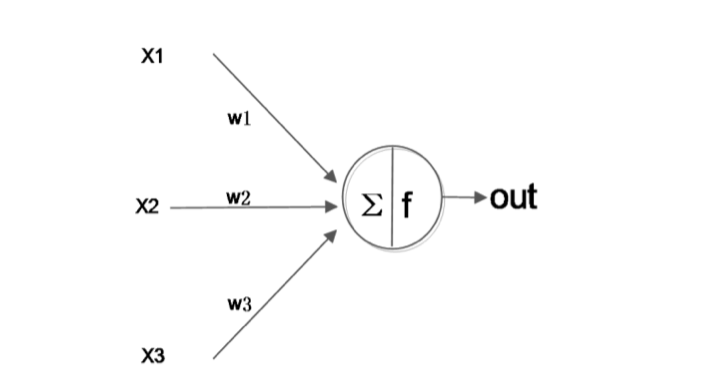
\includegraphics[width=0.7\textwidth]{mlp2.png}
	\caption{basic model of neural unit\label{fig:mlp1.png}}
\end{figure}


As shown in Figure 3.2, it is a network structure of a perceptron model which is composed of two layers of neural networks. 
The input layer receives external input signals and then transmits them to the output layer. 
The output layer is MP neurons. The activation function f of the perceptron is the $sgn$ function, so the perceptron function can be written as:

\begin{equation}
	y=sgn(\vec{w}\cdot \vec{x})
\end{equation}	



\begin{equation}
sgn(y)=\begin{cases}
1 & \text{ if } y>0 \\ 
0 & \text{  } others
\end{cases}
\end{equation}

\vspace{10mm}

The perceptron can be seen as a hyperplane in n-dimensional instance. For instances on one side of the hyperplane, the perceptron outputs 1 and for instances on the other side, 0. The decision hyperplane equation is $\vec{w}\cdot \vec{x}$
The set of positive and negative examples that can be divided by a certain hyperplane is called a linearly separable example set, and they can be represented by a perceptron.\\[2ex]

\begin{figure}[h]
	\centering
	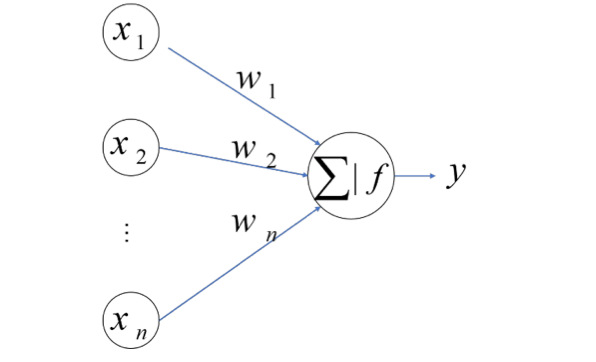
\includegraphics[width=0.6\textwidth]{perceptron.png}
	\caption{basic model of perceptron}
\end{figure}


If the hidden layers are added between the input layer and the output layer, a multi-layer forward network can be formed.
When one layer's neuron is connected to the next layer,  the network is called fully connected. It can handle relatively complex tasks and linearly inseparable classifications. A typical example of this kind of problem is the well-known XOR. As shown in Figure 3.3, it is a three-layer perceptron model. The input has three variables $\left [x_{1},x_{2},x_{3}  \right ]$.
4 neurons in the hidden layer and 2 neurons in the output layer. The following analyzes the process of forward propagation.Firstly, some variable information is defined. 
For the $l$ layer, use all neurons in the layer $L_{l}$ to represent the output $y_{l}$. The output of the j node is $y_{l}^{j}$ and the input of this node is $u_{l}^{j}$. The weight matrix connecting the layer $l$ to the layer $l-1$ is $w_{l}$.The weight of i node in the $l-1$ layer to the j node in the $l$ layer is $w_{l}^{ji}$.


\begin{figure}[h]
	\centering
	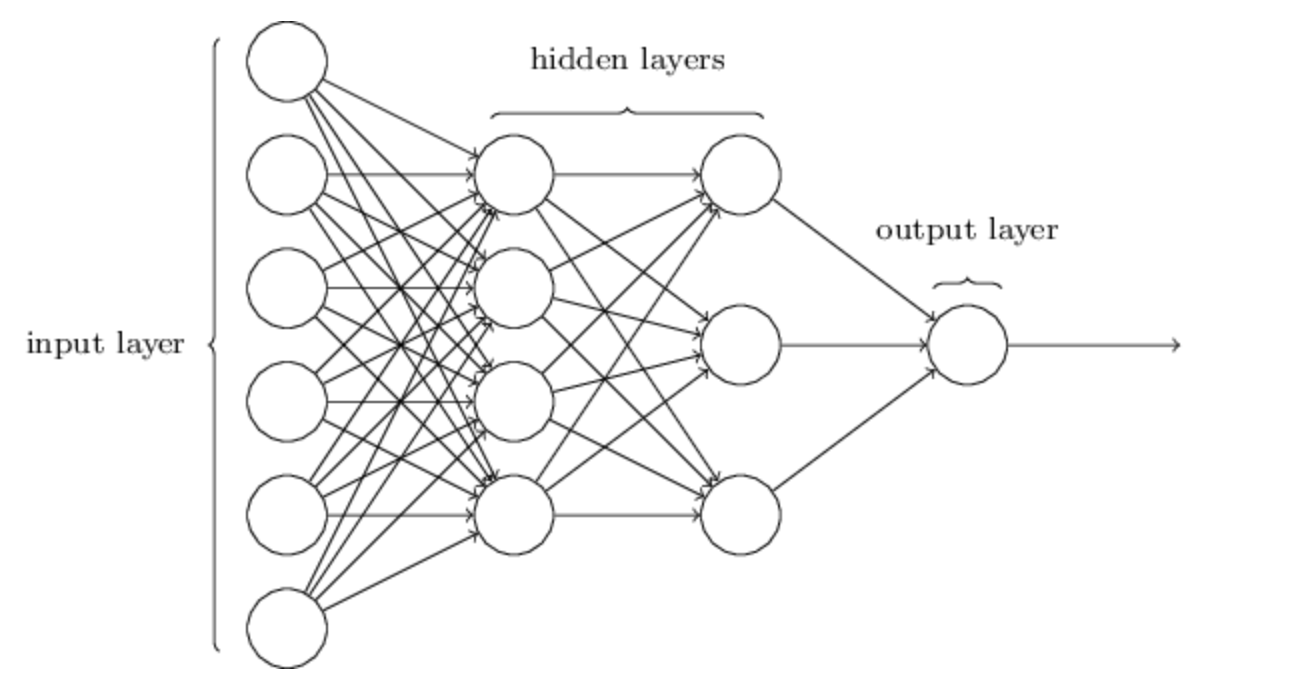
\includegraphics[width=0.7\textwidth]{mlp.png}
	\caption{basic model of MLP}
\end{figure}


\section{CNN}
The rapid development of convolutional neural networks has made great contributions to the problem of improving the accuracy of classification tasks. The concept of sensory field was proposed by Hubel and Wiesel proposed the concept of sensory field in 1962, and further discovered the hierarchical processing mechanism of visual cortex pathway information by studying the visual cortex system of the cat's brain.\cite{cirecsan2012multi} The convolutional neural networks were proposed. CNN is widely used because they can directly input the original image without complex preprocessing.

Convolutional Neural Network (CNN) is a deep network model. Figure 3.4 has the information for CNN. Compared with previous networks, convolutional neural networks are special in two aspects: local connection and weight sharing. Briefly illustrated by the following example.


\begin{figure}[h]
	\centering
	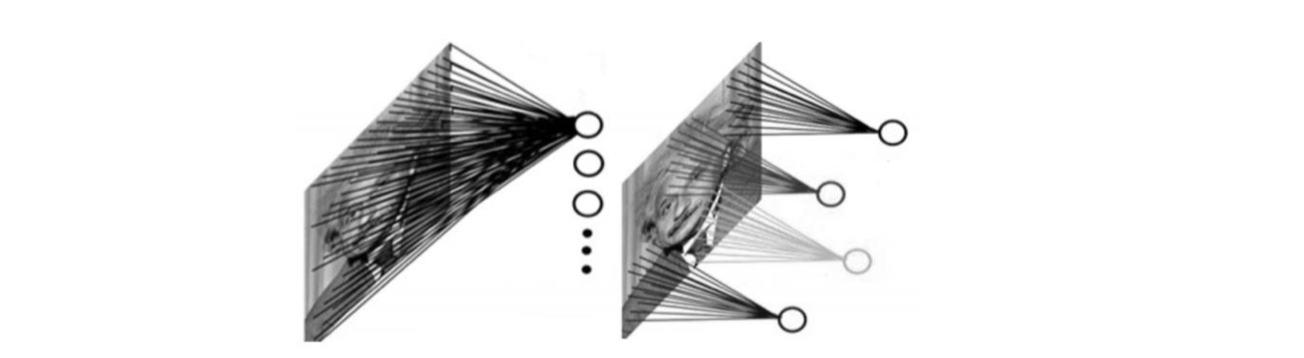
\includegraphics[width=0.7\textwidth]{fullyConnected.png}
	\caption{basic model of CNN}
\end{figure}

Suppose there is a single-channel grayscale image of 10,000x1000 pixels with 10,000 neurons in the hidden layer. As shown in Figure 3.4, in the fully connected network on the left, each pixel in the figure needs to be connected to each neuron once, there are $10^{10}$ connections. In the local connection network on the right, the neurons only need to connect to the convolution kernel. 
Assuming the size of the convolution kernel is 10x10, the parameters connected to the 10x10 region are only $10^{6}$  parameters. Compared with the latter, the parameters in the former are $10^{4}$  of that.

In the interpretation shown by weight sharing, there is an assumption that the size of the convolution kernel is 10x10. In the local connection network shown on the right, each neuron needs a connection weight parameter of 100. If different convolution kernels are used, the weight parameter that each neuron needs to connect is the number of convolution kernels multiplied by the weight parameter of a single convolution kernel. But if each neuron uses the same convolution kernel, then this The network only needs 100 parameters, which is called weight sharing. Weight sharing not only improves the learning efficiency, but also reduces the number of learned parameters.


\subsubsection{structure of CNN}
In machine learning,CNN is a deep feedforward artificial neural network, which can perform image processing with a large dataset. 
CNN is improved based on BP neural networks.\cite{krizhevsky2012imagenet} Both networks use a forward propagation algorithm to calculate the output value, and use a backward propagation algorithm to optimize the offsets and weights . 
The difference between a CNN and a BP neural network is the way the neural units are connected. In the CNN, the neural units between adjacent network layers are locally connected, which is different from the neural unit connection in the BP network. All neural units of the BP network are interconnected. In a CNN, the perceptual area of the neural unit is derived from some of the neural units in the previous network layer. CNN's structure includes convolutional layer, pooling layer, activation layer and fully connected layer.\cite{abdel2012applying}

\subsubsection{convolutional layer}
In a CNN, each convolutional layer consists of multiple feature maps that exist in the form of a second-order tensor. In this network, the weight matrix extracts the features of the image by performing a dot product operation with the input image respectively. One weight matrix corresponds to one feature map. Each convolution operation is a feature extraction method. After each convolution operation, a feature map can be obtained. 
The movement mode of the convolution kernel is determined by the step size of the convolution kernel. The size of the output feature map is determined by the margins (p adding) determines , that is: $L = (L + 2 * padding-kernel size) / stride.$

\subsubsection{pooling layer}
In this network, the pooling layer focuses on reducing the spatial dimension of the collected feature map. Meanwhile, as the pooling layer also scans the image, it also plays a secondary extraction role. 
Max-pooling and mean-pooling are two common pooling methods. 
Main difference between the two is that the former finds the maximum value in the selected area as the value after pooling, while the latter uses the average value.\cite{nagi2011max}

\subsubsection{fully connected layer}
In the CNN, the previous convolutional layer and pooling layer first perform feature extraction and image dimension reduction on the image, and then input it into the later fully connected layer. This layer uses the product of matrix vectors to weight the sum of the input image and classify it, then corresponds the result to the label, and returns the error.

\subsubsection{activation layer}

In the activation layer, the activation operation on input data (non-linear function transformation) is performed element by element.\cite{gomes2004comparison} There are several activation functions, including the Sigmoid function, the ReLU function and the Tanh function. The sigmoid function is shown in formula.


\begin{equation}
	f(x)=\frac{1}{1+e^{-x}}
\end{equation}	
 
The output range of the Sigmoid function is between (0, 1), which is monotonically continuous. The output range is limited  and the optimization is stable.It can be used as an output layer.


The tanh function is similar to the sigmoid function . They both are basically zero mean. Therefore, the tanh function will perform better than the Sigmoid function in practical applications. The function expression is shown in formula.


\begin{equation}
	tanh(x)=\frac{1-e^{-2x}}{1+e^{-2x}}
\end{equation}	

The Tanh function converges faster than the Sigmoid function. Compared to the Sigmoid function, its output is centered at 0. Figure 3.5 is a trend graph of the Sigmoid function and the Tanh function, including the domain and range of values.

\begin{figure}[h]
	\centering
	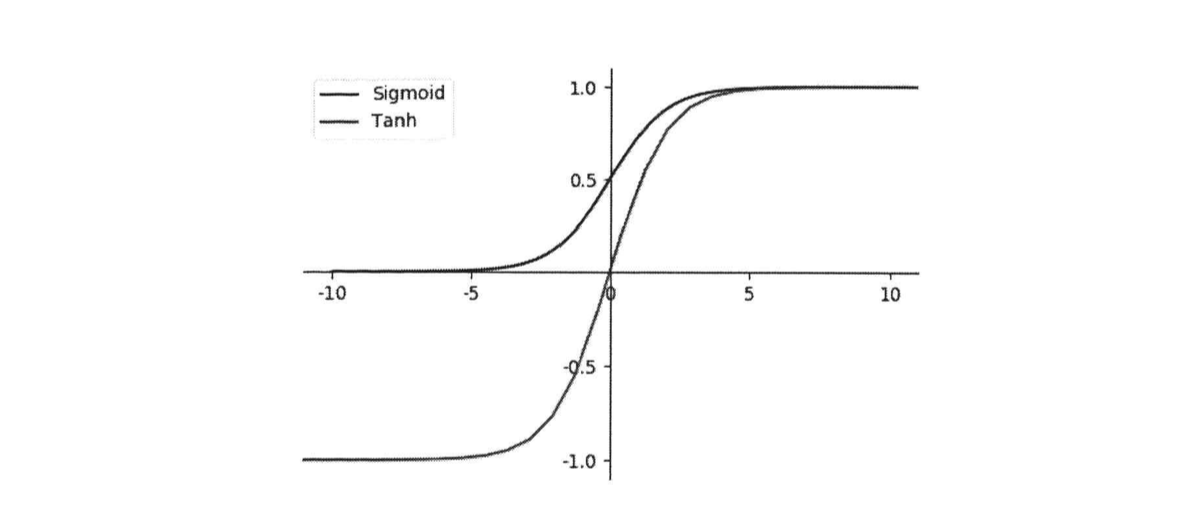
\includegraphics[width=0.7\textwidth]{sigmoid.png}
	\caption{Characteristic curves of Sigmoid and Tanh functions}
\end{figure}

From a mathematical point of view, the Sigmoid function has a larger signal gain for the central region and a smaller signal gain for both sides. In the signal feature space mapping, it has a very good effect. From the perspective of neuroscience, the central region can represent the excited state of the neuron, and the bilateral regions can represent the suppressed state of the neuron. Therefore, in the aspect of neural network learning, the Sigmoid function can move the key features to the central area and the non-key features to the two areas.

In specific applications, the Tanh function is often more superior than the Sigmoid function. The reason is that the Sigmoid function is at the input range [-1, 1], the function value is sensitive to changes. Once approaching or exceeding the defined interval, the function value basically does not change and enters the saturation state, which makes the network prediction accuracy to decrease. The output and input of Tanh can maintain a non-linear monotonic rising and falling relationship, which is in line with the gradient solution of neural network. Tanh has good fault tolerance and it is bounded. Compared to the Sigmoid function, it delays the time to enter the saturation state.

ReLU function is also called Receipt Liner Units, which is a very popular activation function in recent years. It is widely used after the BP algorithm. The function expression is shown in formula (3.6).

\begin{equation}
	y=\begin{cases}
0 & \text{ } x<=0 \\ 
x & \text{  } x>0
\end{cases}
\end{equation}	


The ReLU function is actually a piecewise linear function. Compared with other activation functions, ReLU converges faster and can  express better, especially in the field of deep networks. Figure 3.6 is the characteristic curve of the ReLU function.


\begin{figure}[h]
	\centering
	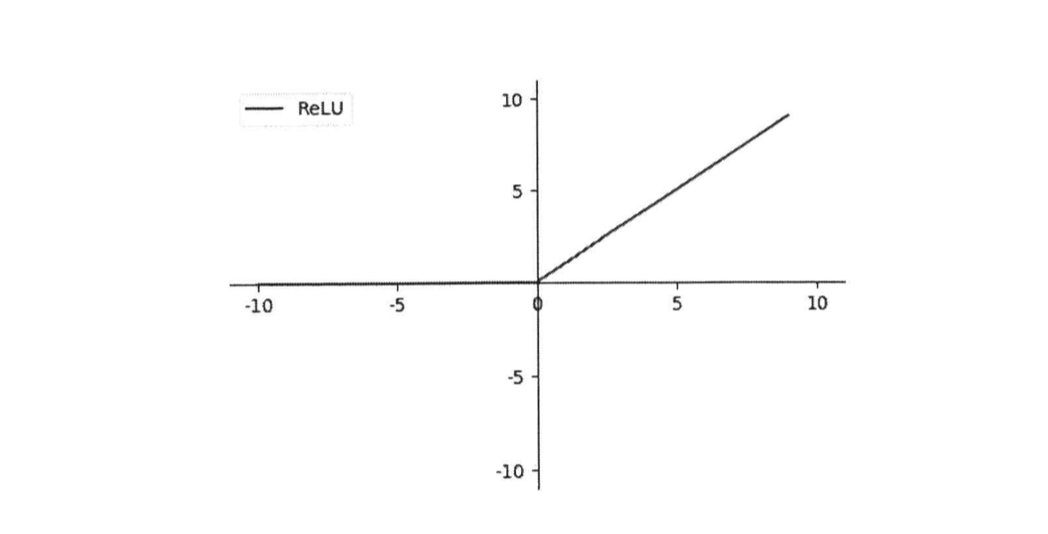
\includegraphics[width=0.7\textwidth]{relu.png}
	\caption{Characteristic curves of relu function}
\end{figure}

 Output of relu is 0 in the negative region and x in the non-negative region. This characteristic is called unilateral suppression. Because of the characteristics of unilateral suppression, neurons in neural networks also have sparse activation, which enables the model to better mine related features and fit training data.
 As the gradient of the non-negative interval of ReLU is constant, there is no vanishing gradient problem (Vanish Grading Problem), which keeps the model in a stable convergence rate .


\section{LSTM}

The long short-term memory network (LSTM) structure was first proposed by Hochreiter and Schmidhuber in 1997.\cite{cheng2016long} The reason why they proposed the LSTM network structure is to be able to deal with the long-term dependency problems faced by traditional RNN networks. As a result, neural networks do not need to deliberately remember Long-term information, but let the network learn a default memory behavior. This solution is to cleverly make articles on neural nodes. By adding forget gates, input gates, and output gates similar to the gated structure, the weights of the neural nodes' self-loops are changed. 
The LSTM network is a modification of the RNN network.\cite{schuster1997bidirectional} It can solve the problem that the RNN network does not handle the long-term dependency problem. The core idea behind its architecture is a storage unit that can maintain its state over time, and control information inflow and outflow units. Nonlinear gating unit. It is currently more popular in dealing with traffic flow prediction. The next section will detail the LSTM network structure and the working principles of each part.

Figure 3.7 shows the structure of an LSTM basic unit. Similar to the RNN, the LSTM unit has a layer input $x_{t}$ and a layer output $h_{t}$  at each iteration. When training and updating parameters, the complex unit also takes into account the unit input state $C_{t}$, the unit output state $\tilde{C_{t}}$, and the previous unit output state $C_{t-1}$

\begin{figure}[h]
	\centering
	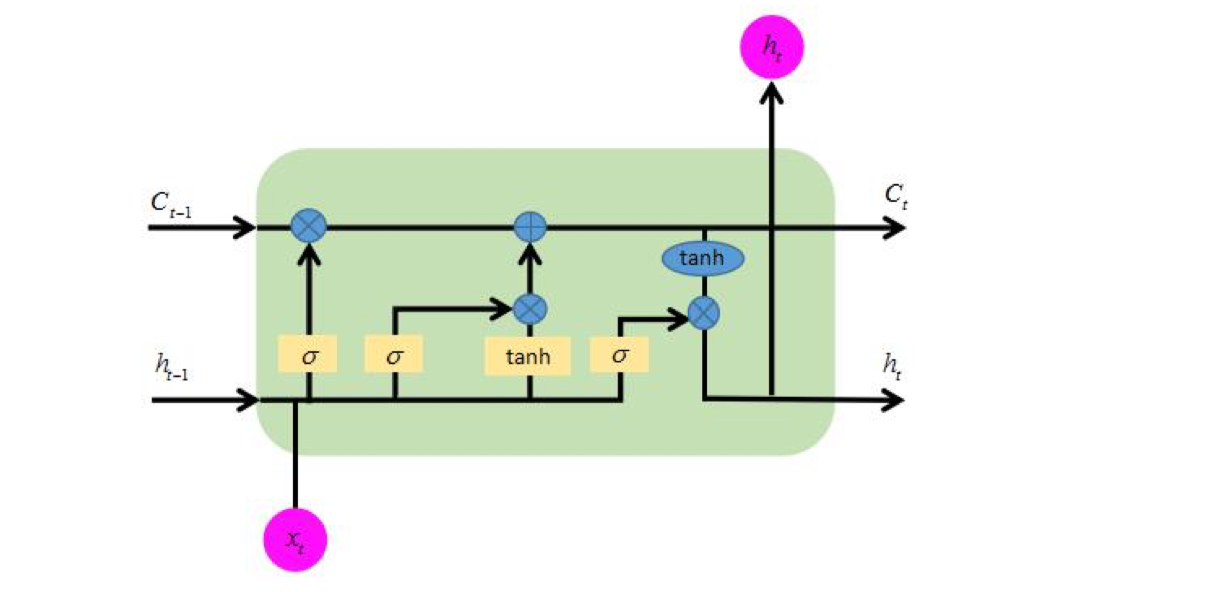
\includegraphics[width=1.0\textwidth]{lstm1.png}
	\caption{The architecture of LSTM}
\end{figure}


In the LSTM, the basic structure of the hidden layer is a storage unit. As shown in Figure 3.7, the structure is an LSTM cell structure unit. 
It contains one or more memory cells and a pair of adaptive, multiplicative connected units that connect input and output to all units in the block. The core of each storage unit has a linear self-connecting linear unit, which is generally called "constant error transfer", and the activation of this unit is called "unit state", which is the key to LSTM. Figure 3.8 shows the constant error transmission of a unit within the dashed box.

\begin{figure}[h]
	\centering
	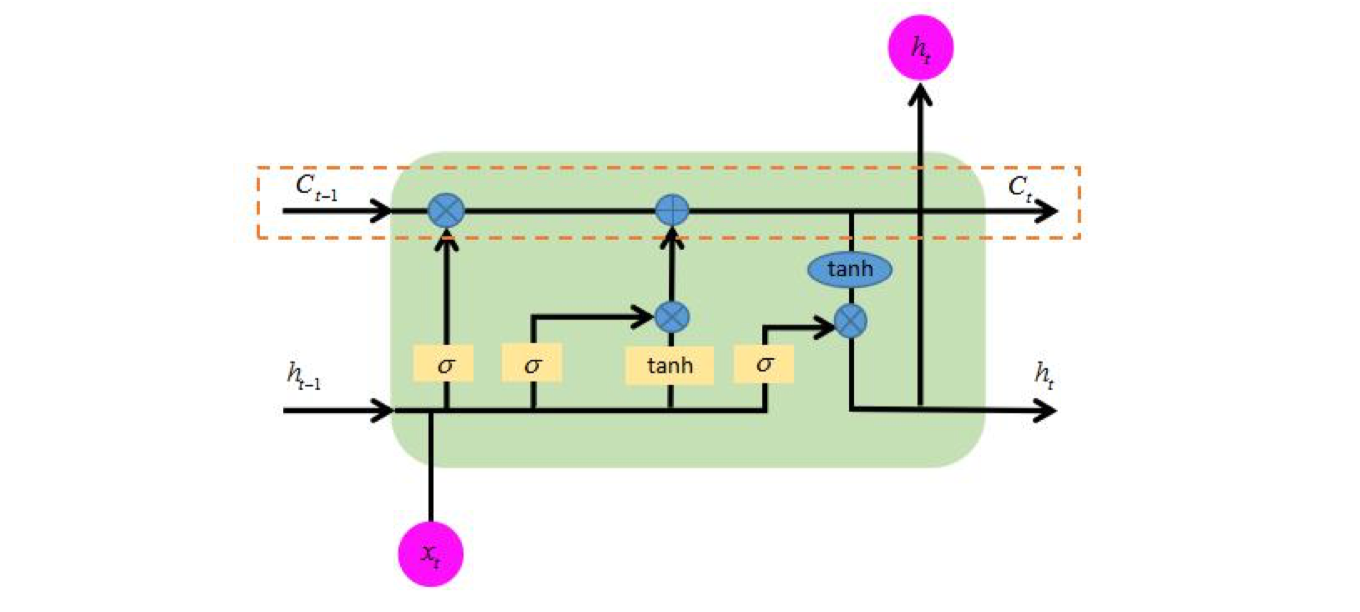
\includegraphics[width=1.0\textwidth]{lstm2.png}
	\caption{Constant error transmission structure}
\end{figure}


Constant error transmission solves the problem of disappearing errors: in the absence of a new input or error signal, the local error return of the constant error transmission remains unchanged, neither increasing nor fading. However, if there is only a constant error conveyor, the LSTM structure cannot add and delete information flow. Therefore, someone has proposed a similar gated structure to realize the filtering in the information transmission process. 
As shown in Figure 3.9, through a neural layer of a sigmoid function and a point-by-point multiplication operation, the gated structure cleverly filters information.
\begin{figure}[h]
	\centering
	
\includegraphics[width=1.0\textwidth]{gate.png}
	\caption{Gate control structure}
\end{figure}

Through the sigmoid layer structure,  an output value between 0 and 1 can be obtained. These output values mean a weight distribution of passing information (for example, 0 means that no information is allowed to pass through the structure, and 1 means that All information passes through this structure).

In summary, the LSTM unit contains three gate structures: forget gate, input gate and output gate. These gated structures, especially forgetting gates, help LSTMs become an effective and well-performed model for solving several sequential related problems. 
For the $t$ time step, the forget gate, input gate, and output gate are denoted as $f_{t}$, $i_{t}$, and $o_{t}$ respectively. The calculation of the state of the forget gate, input gate, output gate, and input unit is indicated by the blue circle in the LSTM unit in Figure 3.7.

Through the following formula, the storage unit can described  in LSTM in detail:

\begin{equation}
	f_{t}=\sigma (W_{f}\cdot[h_{t-1},x_{t}] + b_{f})
\end{equation}	

\begin{equation}
	i=\sigma (W_{i}\cdot[h_{t-1},x_{t}] + b_{i})
\end{equation}	

\begin{equation}
	C_{t}=f_{t}*C_{t-1}+i_{t}*tanh(W_{c}\cdot[h_{t-1},x_{t}] + b_{c})
\end{equation}	


\begin{equation}
	O_{t}=\sigma (W_{o}\cdot[h_{t-1},x_{t}] + b_{o})
\end{equation}	

\begin{equation}
	h_{t}=O_{t}*tanh(C_{t})
\end{equation}	

$i_{t},O_{t},f_{t}$ represents input gate, output gate and forget gate respectively. $C_{t}$ is the state vector of the memory cell.
	$h_{t}$  represents a single unit output vector. $W$ and $b$ represents a weight matrix and a deviation vector.$\sigma$ and $tanh$ functions show as following:

\begin{equation}
	\sigma (x)=\frac{1}{1+e^{-x}}
\end{equation}

\begin{equation}
	tanh(x)=\frac{e^{-x}-e^{-x}}{e^{-x}+e^{-x}}
\end{equation}	
		
		
Similar to the RNN, the parameters of the long-term and short-term memory models are fitted by time back-propagation. The difference is that the gate structure of the long-term and short-term memory models can effectively solve the  gradient disappearance and deal with long-term dependencies in time series problems.
	
	






\chapter{Analysis and Design}
\subsection{Data}
\subsubsection{Data capture}
The dataset of this project has two parts, the sky images and  the corresponding photovoltaic power values.
The sky images and  the corresponding  power values are from the photovoltaic panel which was installed on the roof of EE building in Xi'an Jiaotong University. Sky camera was installed near the solar panel to capture the images. The sky camera capture the sky images from around 8:00 am to 18:00 because the information of the sun can be captured in the images to achieve the purpose of using the sky image to predict. For sky images, 5 images can be captured every 5 seconds at different exposures({34,100,500,1000,2800}ms), which can obtain more detail information than single one. 
However, the image with the  first level exposure can get little sky features and the image with the fifth level exposure is overexposed. Therefore, the project only use the images with second, third and forth level exposures.

The file names of sky images for 10 seconds show as figure 4.1. For the filename $"2019-09-11-09-51-51\_0.jpg", "2019-09-11-09-51-51"$ represents the time information and "\_0" represents the first level exposure(34ms).

\begin{figure}[!ht]
	\centering
	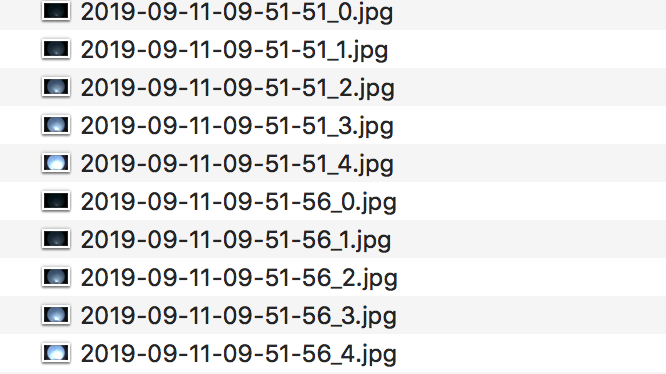
\includegraphics[width=0.45\textwidth]{sun_picture_01.png}
	\caption{file names of sky images\label{fig:sun}}
\end{figure}


In the meantime, solar panel also records the corresponding photovoltaic values into a text file.This precess last for half years. 30 days' information is used in this project.
The figure 4.2 shows the sun and cloud information for the time 2019-09-11-09-51-51.

\begin{figure}[!ht]
	\centering
	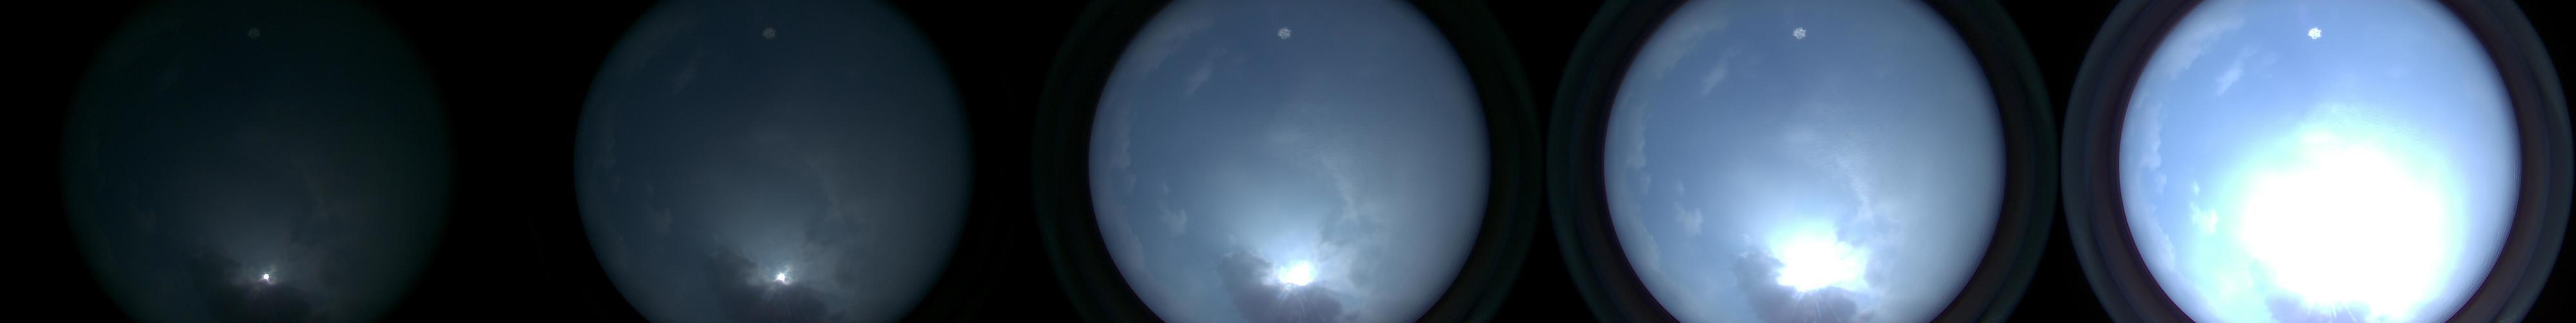
\includegraphics[width=\textwidth]{sun01.jpg}
	\caption{sky images\label{fig:sun}}
\end{figure}

The content of figure 4.3 shows the power values corresponding to the image below.
For the content of figure 4.3, 2019-09-11-09-51-51 represents the time. The value on the right in the picture represents the power value.

\begin{figure}[!ht]
	\centering
	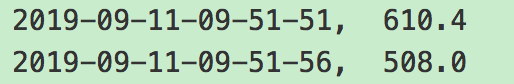
\includegraphics[width=0.4\textwidth]{irradiance_data.png}
	\caption{photovoltaic data\label{fig:photovoltaic}}
\end{figure}


\subsubsection{Data preprocessing}

For power value, the data is collected every 5 seconds. The goal of this paper is to predict the power value after 1 minute through historical data and pictures. Since the historical data is too much, the historical data is simplified to the power value per minute. The problem is transformed into predicting the power value of the next minute by the power value of the previous few minutes. In the process of processing the power value,  power values around 0 are deleted.



For image data, the input of a single CNN network corresponds to a 3-dimensional matrix of $3 \times 4$ channels. (3 exposures in gray scale. A gray scale image only has one channel). The images are taken 1 minute before the current time $t$ with interval 15s. In this way, 4 new images can be obtained every minute.


\subsection{Notation}

For current time $t_{0}$, the power values are defined as $p_{t_{0}}$. For future time $t+t_{0}$,the power values are defined as $p_{t+t_{0}}$. As this work focuses on the 1-min forecasting, t is on the order of 1 min. The aim of this work is to learn the future power output $\hat{p}_{t+t_{0}}$. The notation "hat" is to define the estimated values rather than the ground truth. 

Several new constructed neural network models are used to predict $p_{t+t_{0}}$ based on the current and the former power values.
	$\mathbf{p}=[{ p_{t_{0}-k}, ... , p_{t_{0}} }]$

\begin{equation}
	\hat{p}_{t+t_{0}}=f(\mathbf{p};W)
\end{equation}
 
$W$ represents a set of trainable weights in the network $W=[W_{1}, ... , W_{L}]$, where L represents the number of layers.

The set $\phi$ is used to define the current and past images as $\phi =[I_{t_{0}-k}, ... , I_{t_{0}}]$. The inputs of new constructed network are the sky images $\phi$ and the corresponding power values $\mathbf{p}$. The aim of this network is to predict the future power output $\hat{p}_{t+t_{0}}$.

\begin{equation}
	\hat{p}_{t+t_{0}}=f(\mathbf{p},\phi;W)
\end{equation}





\subsection{DESIGN OF THE PROPOSED ALGORITHM}


\subsubsection{MLP}
MLP(multi-layer perceptron) are comprised several neuron layers. Data is the input for the input layer. In the middle of the network, there can be several hidden layers. The output layer has the predictions.Here is the structure of MLP.

\begin{figure}[!ht]
	\centering
	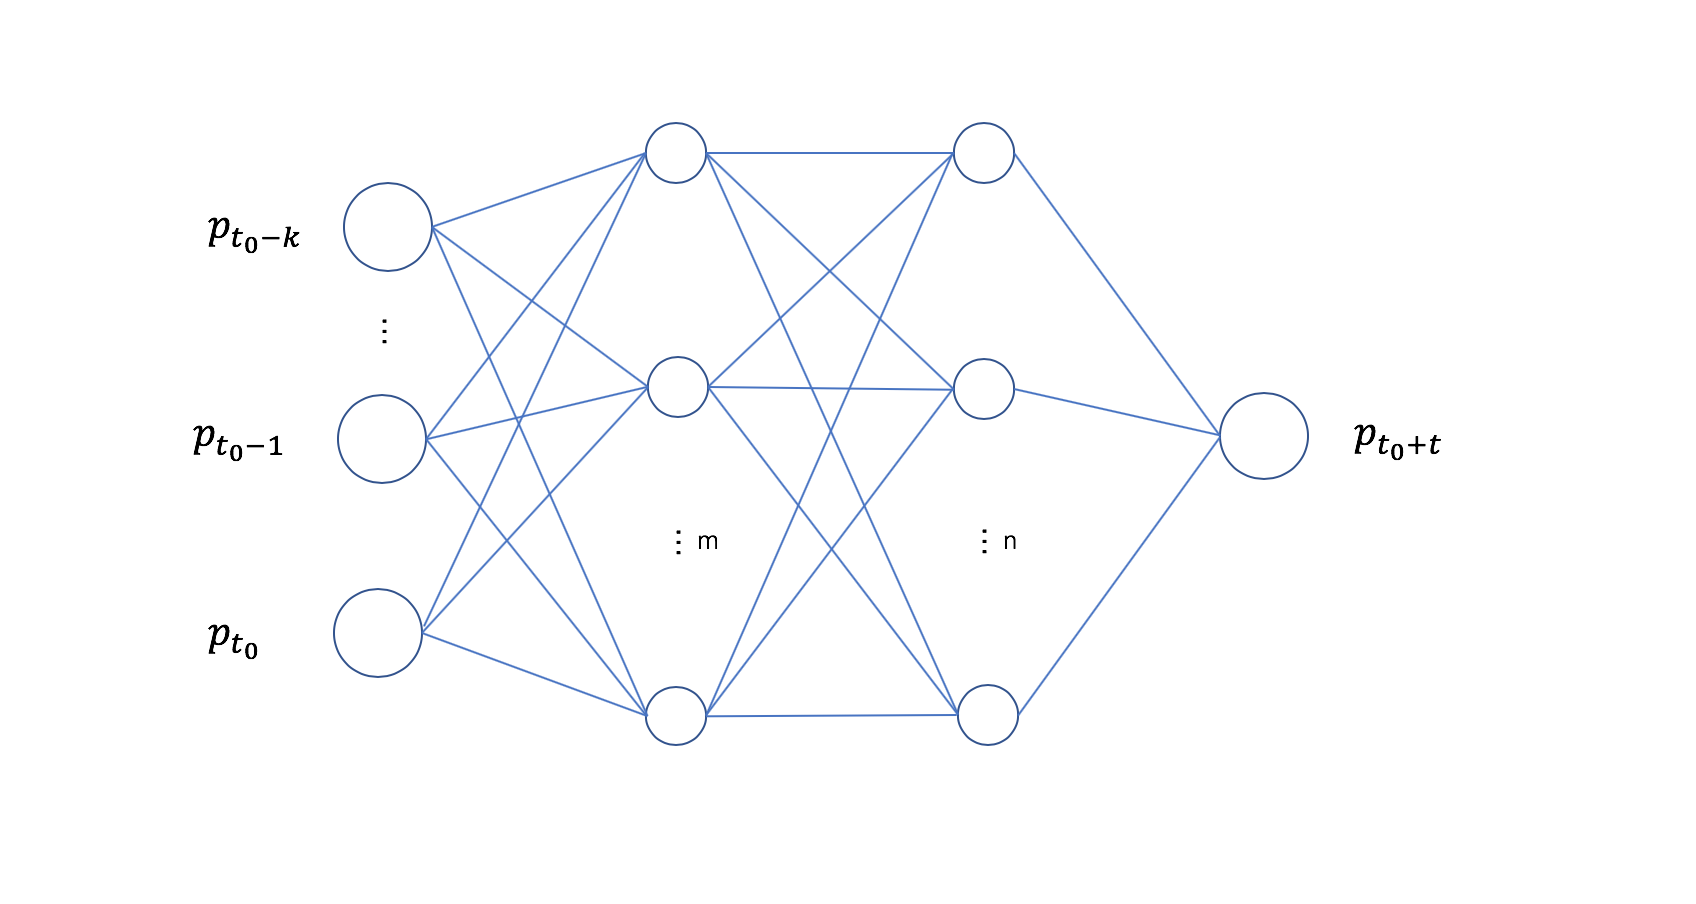
\includegraphics[width=\textwidth]{mlp1.png}
	\caption{basic MLP structure\label{fig:mlp}}
\end{figure}



The input of this model is historical power values, which is noted as $\mathbf{p}$ to predict the future value $\hat{p}_{t+t_{0}}$. This $m\times n \times 1$ MLP network has two hidden layers $m$ , $n$ and one output layer. The value $m = n = 128$ performs well in this network. After these two hidden layers, normalization, the “tanh” activation function are used.Since it is the problem for regression, in the output layer, the network uses “sigmoid” activation function. L2 distance is applied to minimize values between the estimated values and the ground truth.

\begin{equation}
	L_{ p_{t0}}=\left \| \hat{p}_{t+t_{0}}- p_{t_{0}} \right \|  ^{2}
\end{equation}


\subsubsection{CNN}

Although MLP network can use historical power value $p$ as input to do prediction, it has no relevance with images. The procedure does not have enough feathers to feed the model. Therefore, convolutional neural network(CNN) will be applied in order to solve this problem.  CNN is an appropriate model to extract pictures' information. Then this project uses CNN combined with MLP to learn information through the images and  photovoltaic values. Here is the structure of CNN.\\[2ex]


\begin{figure}[!ht]
	\centering
	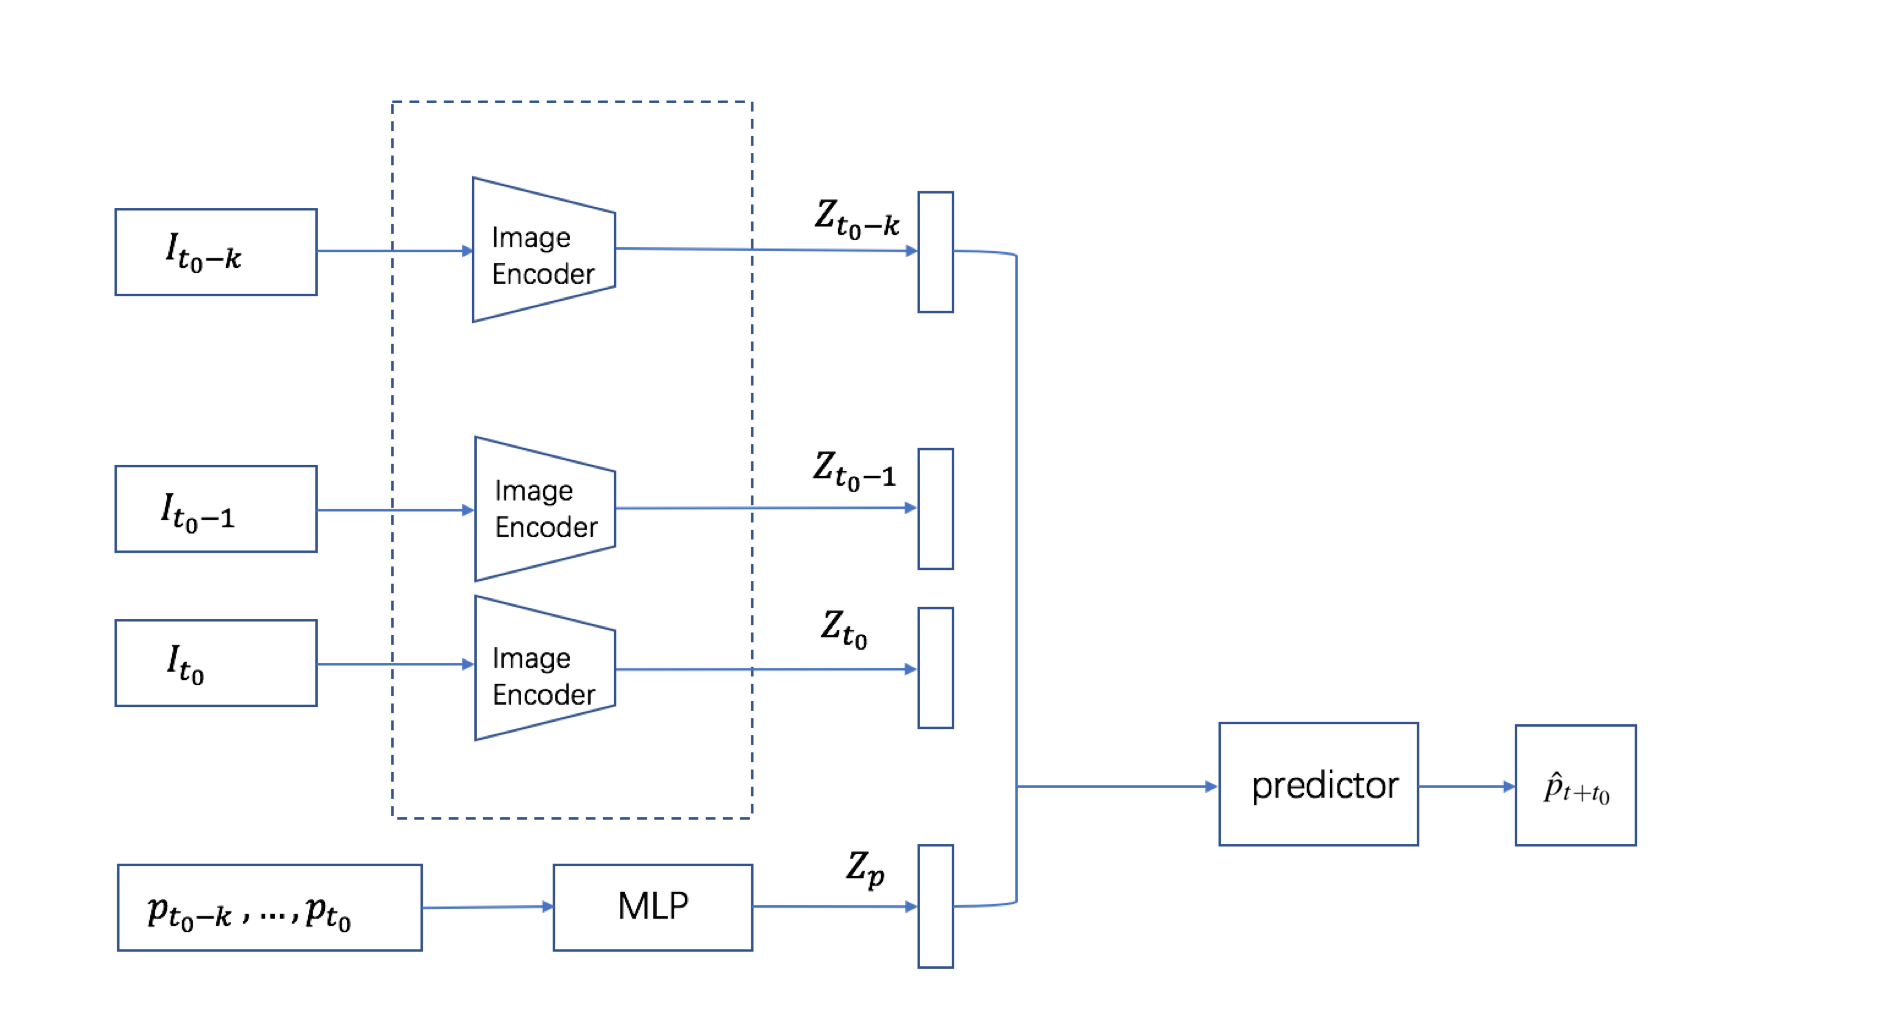
\includegraphics[width=1.0\textwidth]{cnn_mlp.png}
	\caption{CNNs structure\label{fig:cnn_mlp}}
\end{figure}

The image encoder takes 2D image vector as input. After two convolutions, the image information is compressed into a vector $Z_{i}$. There are 6 filters in this network. Besides, there are 3 pooling layers, which uses $2\times2$ max pooling with $stride = 2$ and $kernel size = 2 * 2$.Here is the structure of Image encoder.

\begin{figure}[!ht]
	\centering
	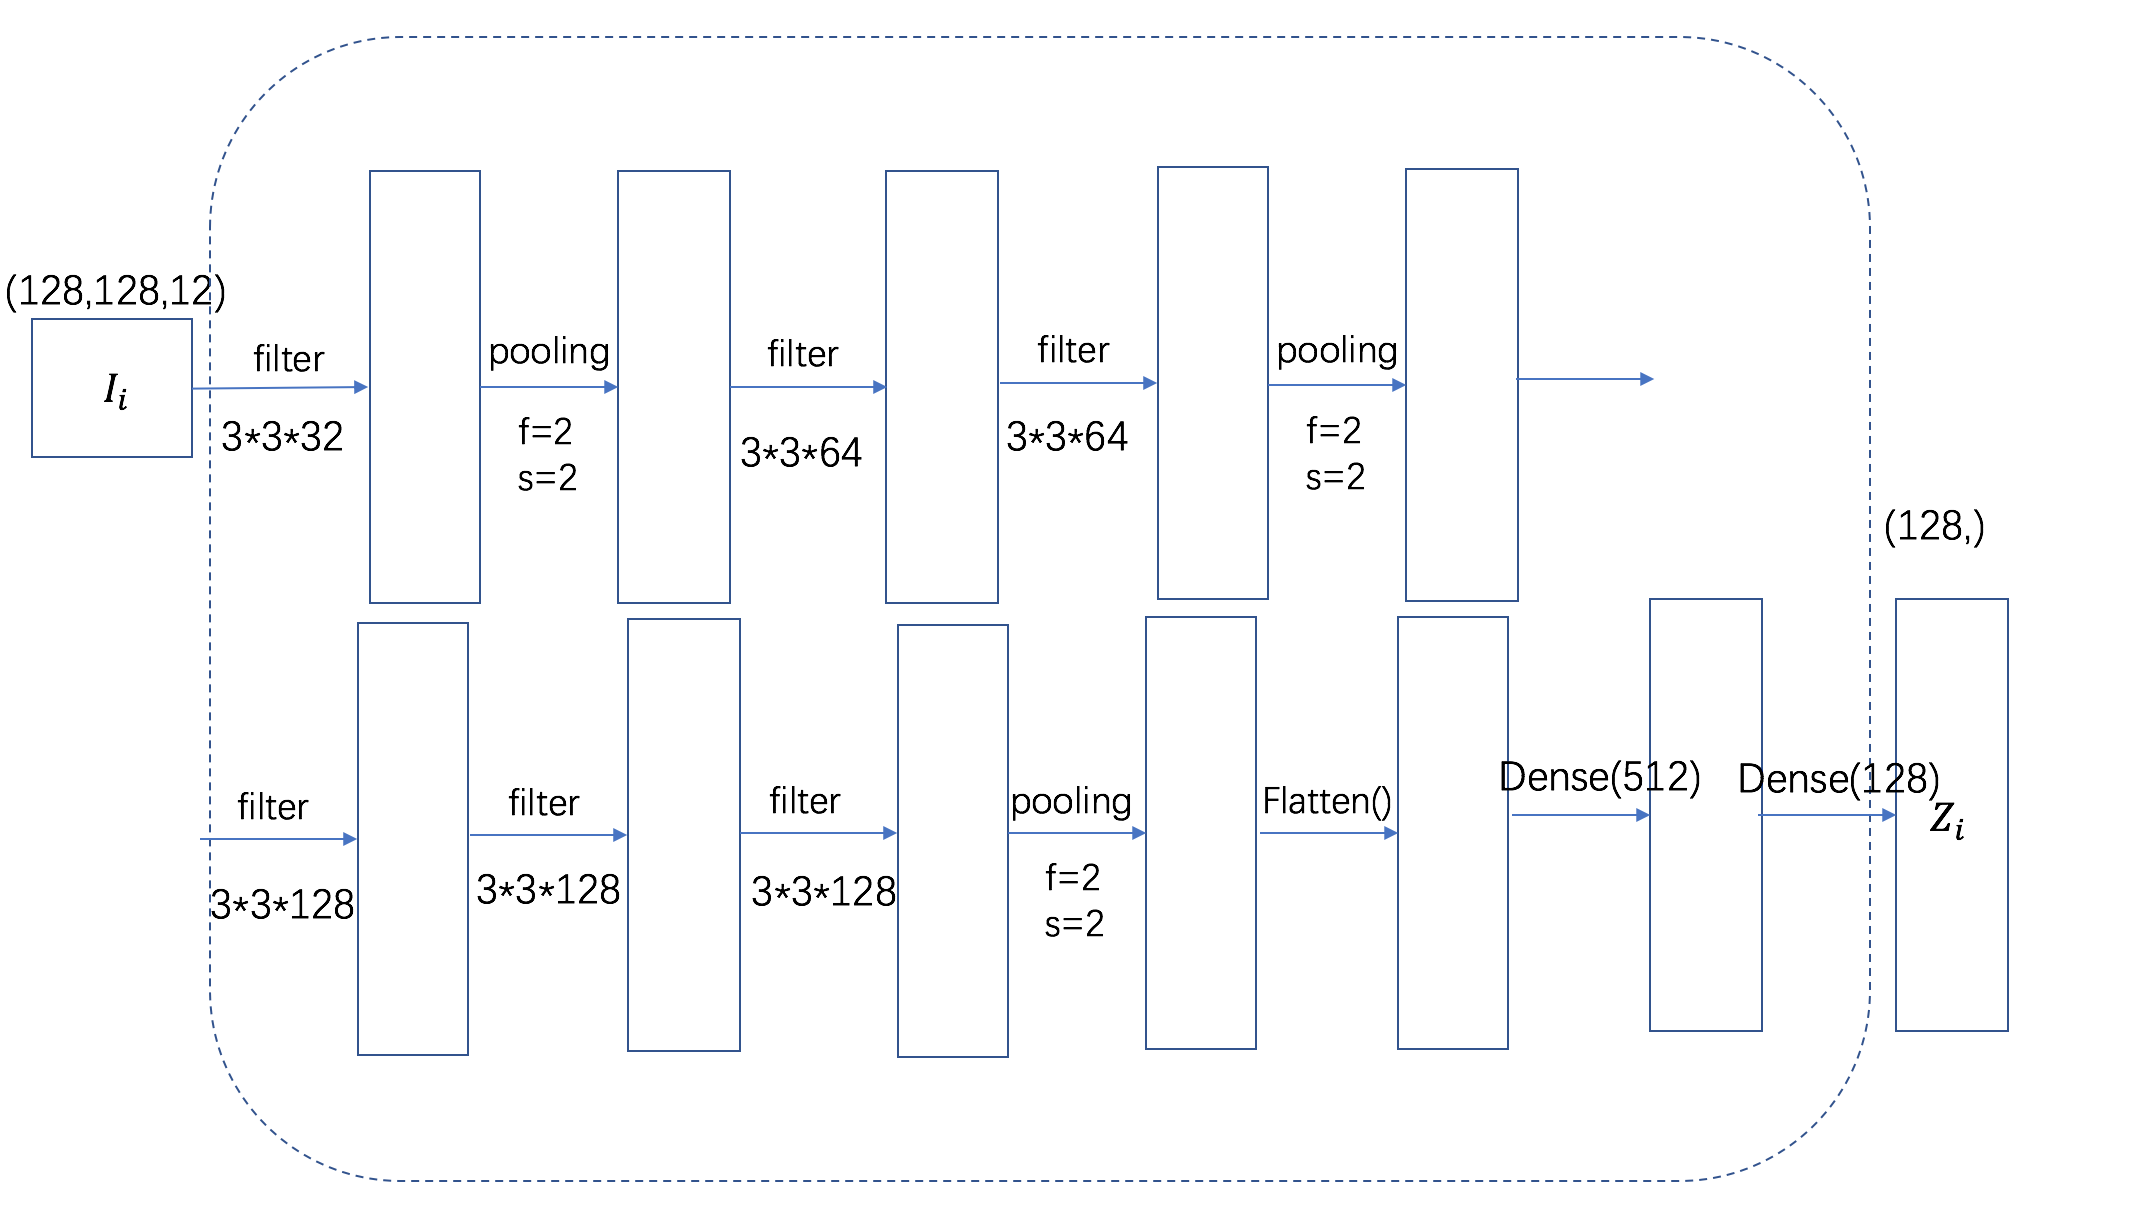
\includegraphics[width=1.0\textwidth]{predictor.png}
	\caption{Image encoder structure\label{fig:Image encoder}}
\end{figure}



The combination architecture contains 2 parts, MLP which has mentioned in last chapter and CNN part. For CNN part, images $I_{i}$ are taken as input, after which the input data is transformed into vector $Z_{i}$ through Image encoder. $i\in \left \{ t_{0}-k, ... , t_{0} \right \}$ Each image will use same set of weights. Power values will be transformed into $Z_{p}$ by MLP. $Z_{p}$ and $\left \{ z_{t_{0}-k}, ... , z_{t_{0}} \right \}$ are fed to the predictor. The predictor can be seen as another MLP network. Its structure is $n \times n \times 1$ with 2 layers. The combined model aims to learn the spatial and temporal changes so as to make precise prediction $\hat{p}_{t+t_{0}}$.\\[2ex]


\subsubsection{LSTM}

The CNNs model takes the image information and power values into consideration, however, temporal information does not take into consideration. In this part, temporal information will be used as another feather to feed the model.

For LSTM network,  $z_{t_{i}}$ are no longer the vectors used into feed the model. Instead, the 1-layer LSTM network is applied in the algorithm architecture. Here is the structure of LSTM.

\begin{figure}[!ht]
	\centering
	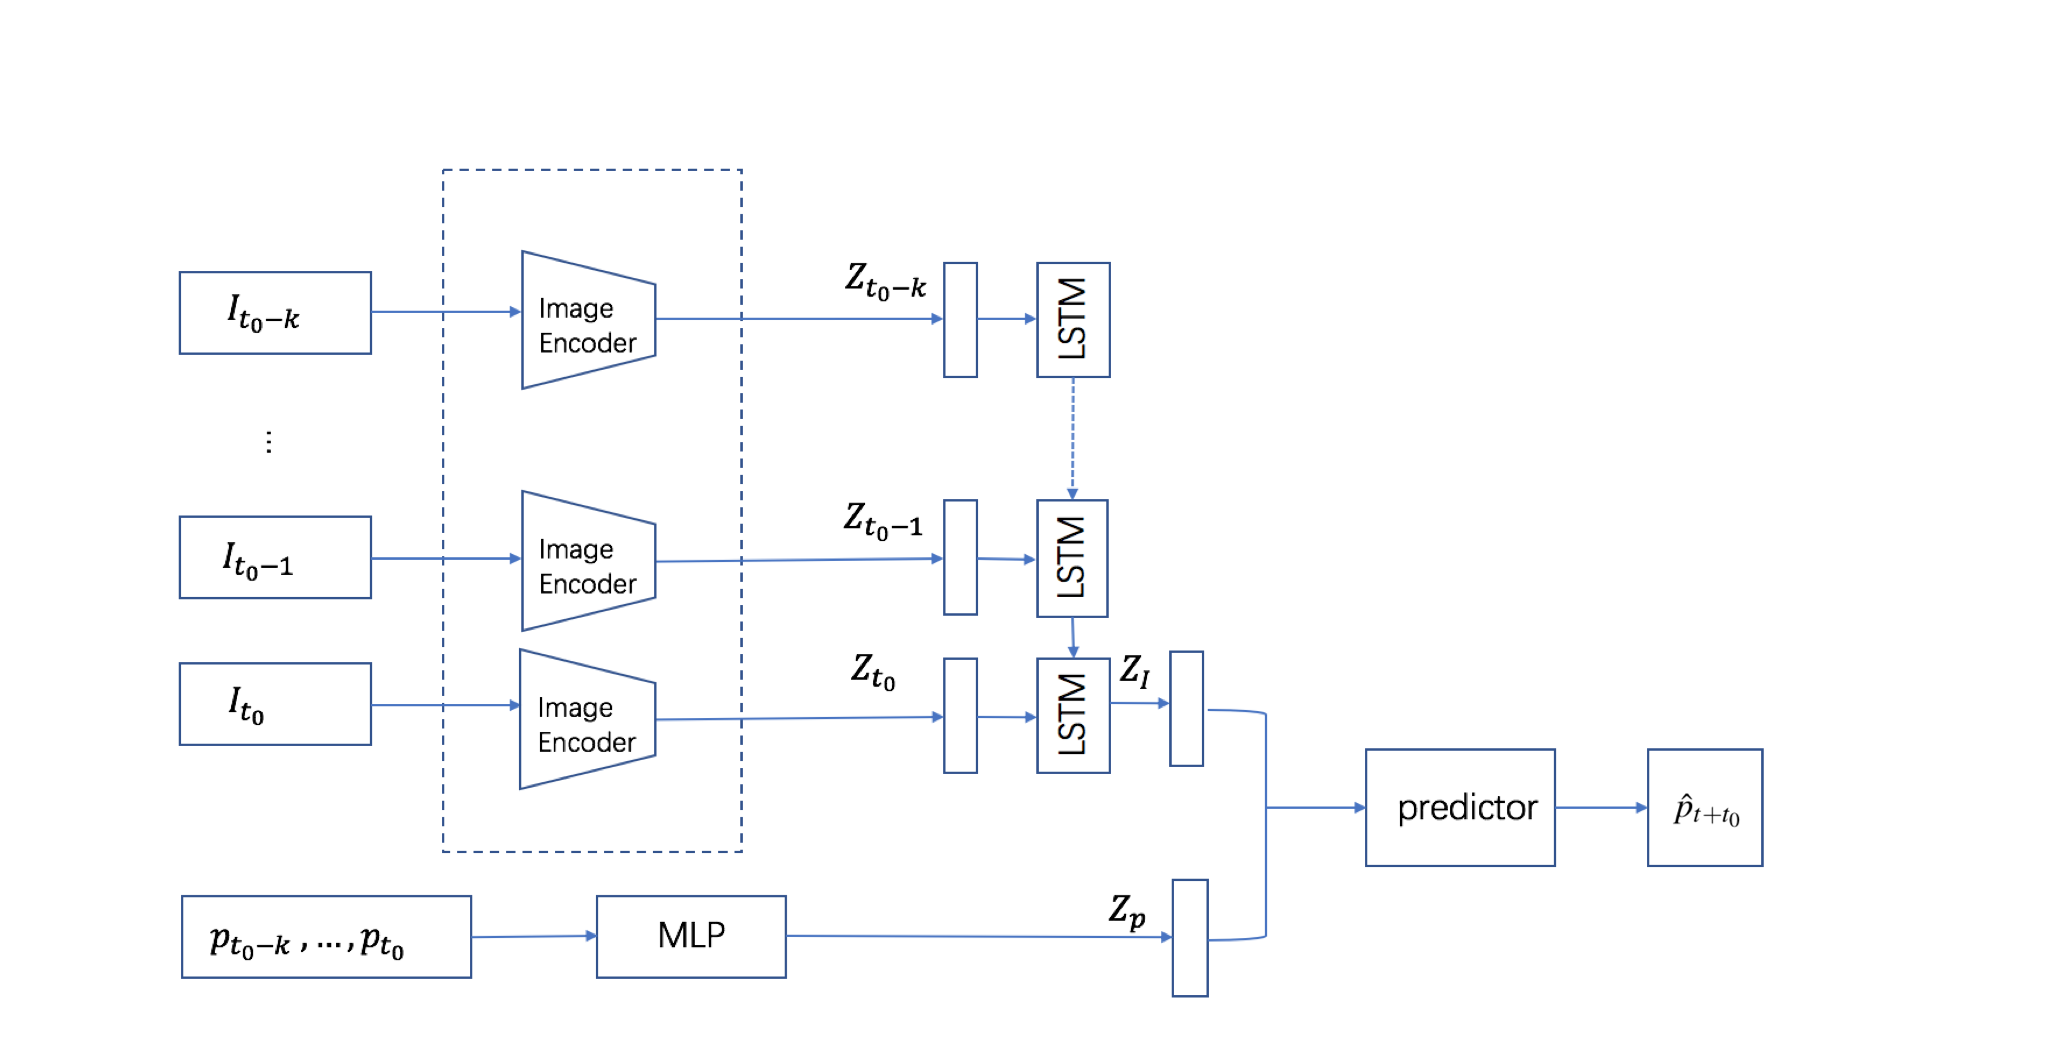
\includegraphics[width=1.2\textwidth]{lstm.png}
	\caption{LSTMs structure\label{fig:lstm}}
\end{figure}

LSTM is good at getting the structure of sequences. After the data being processed, $z_{t_{I}}$ has all the past latent temporal information. Then $z_{t_{I}}$ and $z_{t_{p}}$ are concatenated to train the final network through a predictor to predict  $\hat{p}_{t+t_{0}}$. The loss function remains the same as CNNs.


\begin{equation}
	L_{ p_{t0}}=\left \| \hat{p}_{t+t_{0}}- p_{t_{0}} \right \|  ^{2}
\end{equation}




\subsubsection{Loss function}

The loss function is used to estimate the inconsistency between the predicted value f(x) of the model and the real value Y.\cite{zhu2014novel}
If the result of  loss function is small, the robustness of the model works well. As a core part of empirical risk function, it is an important part of structural risk function.These three models above all use mean squared error(mse) as the loss function.

Mean squared error is the mean of the sum of squares of errors corresponding to the predicted data and the original data. The formula shows as below. $y_{i}$ represents the ground truth.$\hat{y_{i}}$ represents the estimated value.

\begin{equation}
	MSE=\frac{1}{n}\sum_{i=1}^{m}w_{i}(y_{i}-\hat{y_{i}})^2
\end{equation}




% {Documentation of the analysis and design containing full details of the design. The design documentation should also be supplied (possibly as an appendix).}

\chapter{Methods and Realization}

\subsection{Experimental environment}

Deep learning processing image-related problems requires computer support with good enough performance, which requires GPU support. This paper uses a deep learning cloud server.Specific configuration shows as follows. 

Hardware environment:

(1) GPU: One NVIDIA GTXl080ti graphics CARDS.

(2) CPU: E5 CPU processor with 16 threads. 


Software environment:

(1) This experiment is based on Linux system ubuntu 18.04.

(2) This experiment installed the CUDA9.0 computing platform, which enabled the architecture graphics processing unit to solve complex computing problems. In addition, this project uses the GPU acceleration library of CUDNN network.

(3) deep learning framework Keras 2.2.4 and tensorflow 1.12 are installed based on the above environment for fine-tuning the model.   Version 3.1 Opencv is installed, which can realize the diagram like many general algorithms in processing and computer vision. 

This experiment uses the Keras framework to build the overall network.


\subsection{Data preprocessing}

The procedure for data preprocessing shows as follows: First, the time of day when the photos start to be taken is obtained. Then the corresponding power value can be obtained according to the acquired time of taking pictures every day. Photos from 8:00 to 16:00 and power value information are selected, because daily photos are generated from around 8:00 in the morning, and sunlight information after 16:00 is not rich enough.  The daily power values and photo information are saved in the list. In the list, the photos are resize to size of 128*128, which are converted to 1-dimensional gray pictures. The photos at the level of 2,3,4 exposures are selected every 15 seconds. Then 12 pictures in one minute are merged into channels to generate a new picture. This project uses 5 min data to predict next minuate power value. Therefore, one set of power values has 6 min data. First 5 min values are the input of MLP. The last is the ground truth of the network.

Training dataset and test dataset are spilt into 4 categories according to the different weather condition manually: clear, partly cloudy and overcast, all included.


\subsection{Standardization}
Before training the model, all power values are divided into training set and test set randomly. In order to unify the standards and ensure the reliability of experimental results, it is generally necessary to pre-process the original data before modeling, which is commonly referred to as standardized data processing.The original data  need to convert  into dimensionless standardized values to eliminate the effects of different attributes on different indicators, so as to make the results more comparable. Otherwise, the accuracy of experimental results may be affected.

The commonly used data normalization methods include min-max scaling, z-score normalization, linear scaling and so on. In this experiment, min-max normalization method is mainly used to normalize the original data of traffic flow.

\begin{equation}
	X'=\frac{X-X_{max}}{X_{max}-X_{min}}
\end{equation}

\begin{equation}
	X=2\times X' - 1
\end{equation}


$X_{max}$ is the max value in the dataset. $X_{min}$ is the minimum value in the dataset. Through the formula 5.2 , X' scales to a value between -1 and 1.



\subsection{Detail of Experiment}
For MLP part, the network adds dropout layer to prevent overfitting. 

For CNNs and LSTMs, in the training phase, 5 new images which have already been preprocessed is input into the network model. Epoch training is used according to the actual training speed. 
In the parameter setting stage, in order to facilitate the comparison of experimental results, the learning rate was set to 0.001. While training models, each is trained separately with 120 epochs of training. The training process updates the network parameters according to the Adam so that the model reaches the optimal solution. The learning decay rate is 0.001/120.
The experiments use the output of the sigmoid activation function to predict the future 1-min power value.




\subsection{Error metrics}
Root Mean Square Error(rmse) is the square root of the ratio of the square of the deviation of the observed value from the true value to the number of observations m.
RMSE is good at measuring the distance between the ground and the observed value.\cite{willmott2005advantages}

\begin{equation}
	RMSE=\sqrt{\frac{1}{N}\times \sum_{i=1}^{N}(p_{i}-\hat{p}_i)^2}
\end{equation}


Mean Absolute Error(mae) is the average of the absolute errors. The real prediction error can be revealed clearly.\cite{chai2014root}

\begin{equation}
	MAE=\frac{1}{N}\times \sum_{i=1}^{N}|p_{i}-\hat{p}_i|
\end{equation}

RMSE is equivalent to L2 norm but MAE is equivalent to L1 norm. 
The higher the number of times, the more the calculation result is related to the larger value and smaller value is ignored in the meantime. 
Therefore, when dealing with the problem of outliers, RMSE performs better than MAE.

In order to compare the 2 methods' performances, “forecast skill score”(SS) is applied.


\begin{equation}
	SS=(1-\frac{\delta prediction}{\delta  baseline})\times 100 \%
\end{equation}

For the equation above, $\delta*$ represents the error metric to evaluate networks' performance. The baseline represents the suppose that the 1-min future power value is the same as the power value at current time.If the skill score is higher than others, the performance for this model is better.


% {How the design was implemented? Changes made to the design in the course of the implementation. How was the data collected? How was the implementation tested? Typically code listings, screen shots and test runs will appear as appendices}


\chapter{Results and Evaluation}

In the experiment, there are 4 different types of datasets based on the different weather conditions(clear, partially cloudy, overcast). The last type of dataset includes all weather conditions.

For the weather condition, partially cloudy is harder to predict than others because of the unpredicted position of the cloud against the sun. The curve  of training loss and accuracy in  MLP networks show as below. The red curve represents the training loss and the blue curve  represents the test loss. Horizontal axis represents the time of epochs and the vertical represents the loss of the current of the network.
With the increase of time of epochs, the training loss and test loss decrease continuously. However, the two curves do not overlap, which shows that the prediction effect of this network is mediocre.

\begin{figure}[!ht]
	\centering
	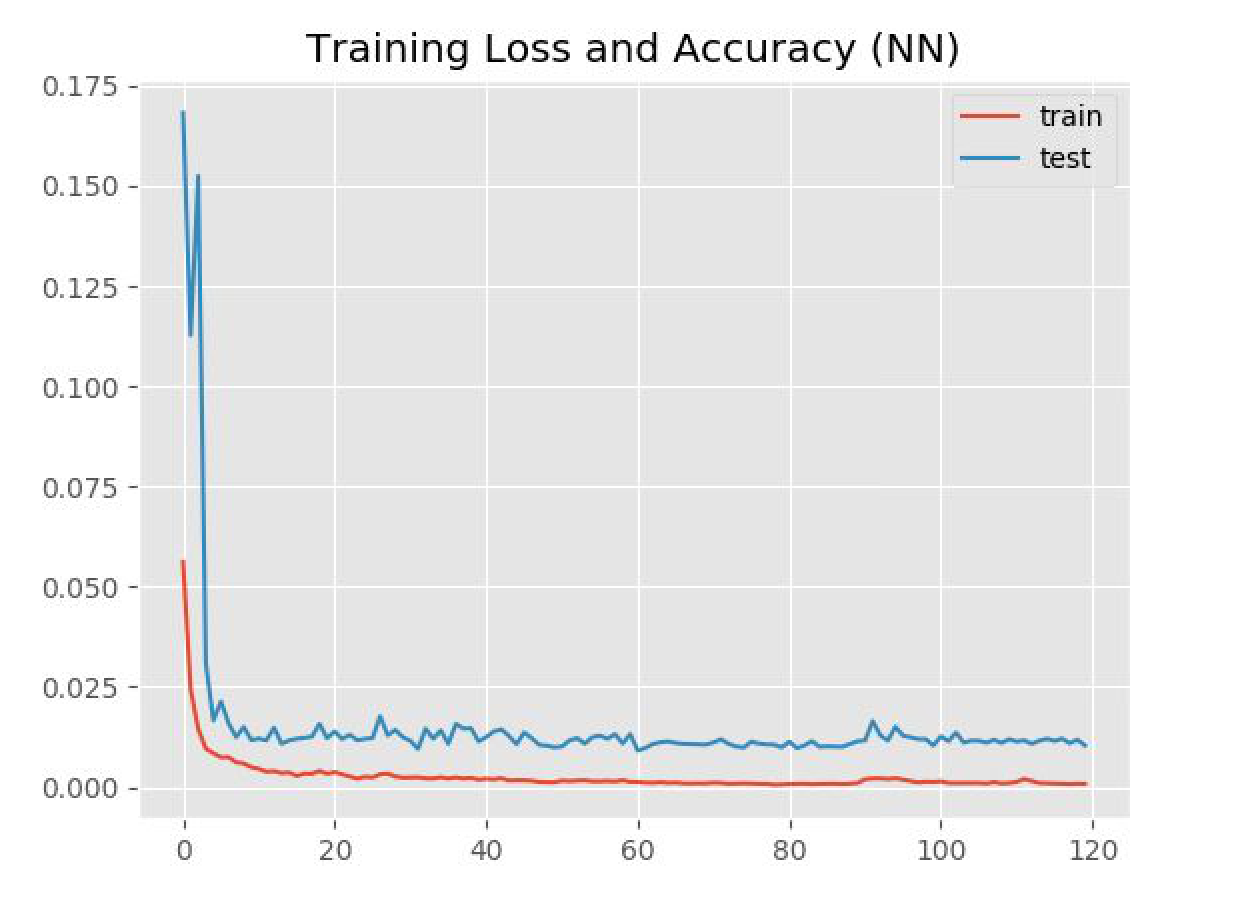
\includegraphics[width=0.8\textwidth]{mlp_acc.png}
	\caption{MLP accuracy\label{fig:mlp}}
\end{figure}

For partially cloudy, the curve  of training loss and accuracy in  CNNs networks show as below. Although high at the beginning, the training loss and test loss decrease continuously. The distance between 2 curves is small in the end of epochs, which indicates that the performance of training network is pretty good. 

\begin{figure}[!ht]
	\centering
	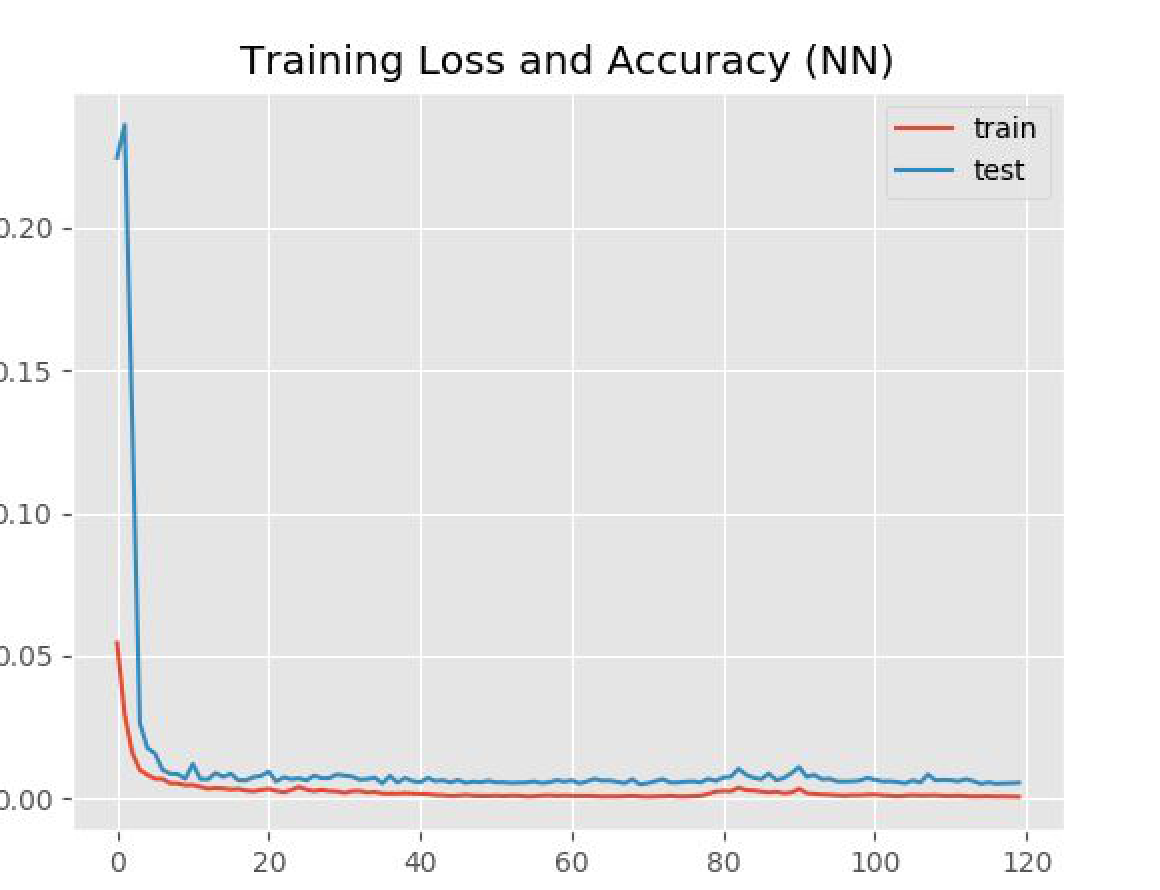
\includegraphics[width=0.8\textwidth]{cnn_acc.png}
	\caption{CNNs accuracy\label{fig:cnn}}
\end{figure}

For partially cloudy, the curve line of training loss and accuracy in  LSTMs networks show as below. The training loss and test loss decrease continuously. The distance between 2 cures is smallest in these 3 networks, which indicates that the performance of training network is the best. 

\begin{figure}[!ht]
	\centering
	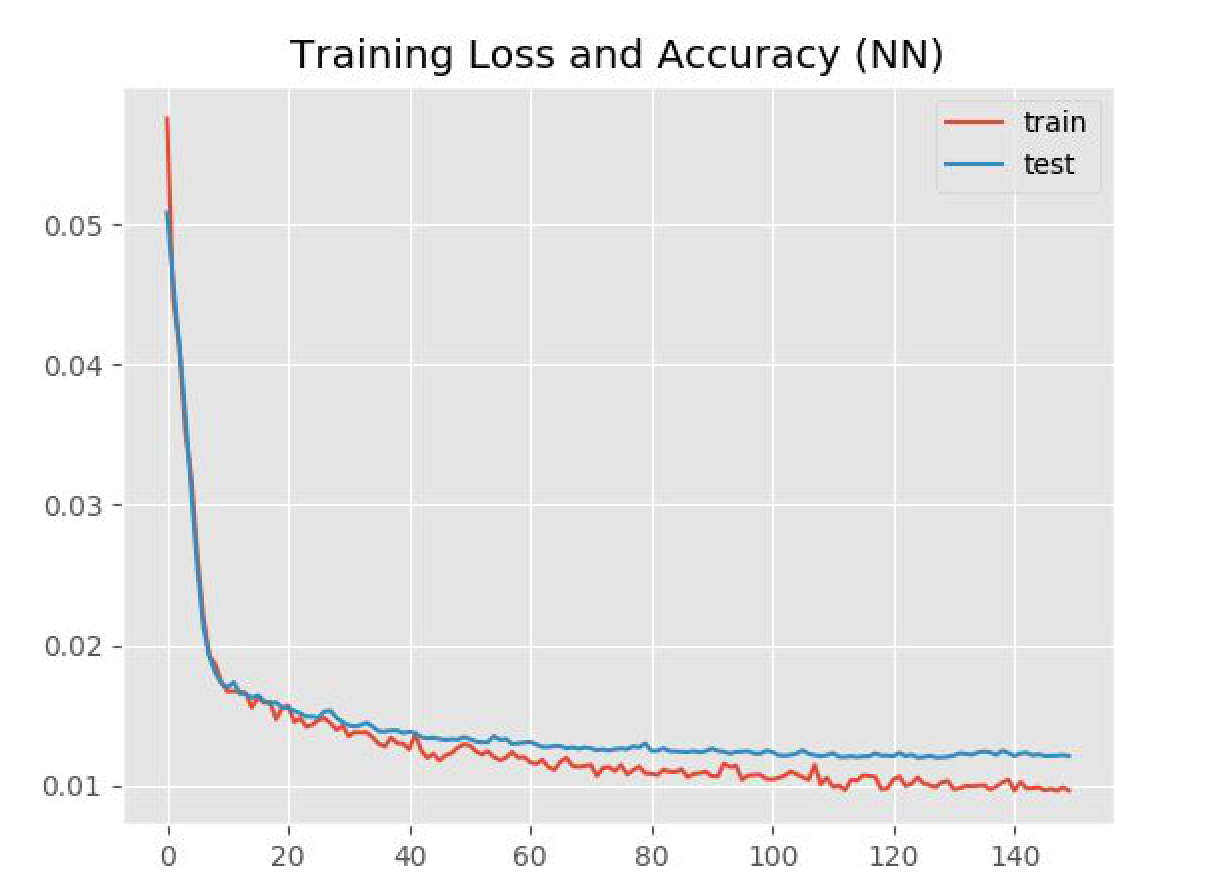
\includegraphics[width=0.8\textwidth]{lstm_acc.png}
	\caption{LSTMs accuracy\label{fig:lstm}}
\end{figure}


Then the 1-min prediction value of mae and rmse is  summarized. The result shows as table 6.1.

%\begin{center}
\begin{table}[h]
\centering
\caption{value of prediction for 1-min future.}
\begin{tabular}{|l|l|l|l|l|l|l|l|l|}
\hline
      & \multicolumn{2}{l|}{clear} & \multicolumn{2}{l|}{cloudy} & \multicolumn{2}{l|}{overcast} & \multicolumn{2}{l|}{all} \\ \hline
      & mae          & rmse        & mae          & rmse         & mae           & rmse          & mae        & rmse        \\ \hline
MLP   & 18.33        & 32.19       & 97.41        & 180.32       & 44.23         & 88.24         & 68.12      & 133.32      \\ \hline
CNNs  & 17.76        & 30.37       & 90.10        & 169.21       & 37.31         & 76.77         & 64.55      & 121.23      \\ \hline
LSTMs & 15.66        & 28.75       & 87.31        & 160.39       & 35.33         & 69.12         & 62.71      & 119.89      \\ \hline
\end{tabular}
\end{table}
%\end{center}

For the 4 different situations, MAE and RMSE of MLP are the highest, which indicates the performance of MLP is not good in these 3 models. On the contrary, MAE and RMSE of LSTMs are the lowest. The MAE indicator reaches  15.63, 87.31, 35.33, 62.71 and the RMSE indicator reaches  28.75,160.39,69.12,119.89.It shows that the network LSTMs works well. The prediction of LSTMs is the most accurate among these three models. MAE and RMSE of CNNs are better than the MLP, which means CNNS is of great help to improve accuracy.


For 1-min forecasting work, the different structures of 3 network models compare with the persistence model. The figure 6.4 shows the concrete values of different models' skill scores for different weather conditions. The higher the value is, the better the performance of model will be.The figure 6.5 shows the detail information of RMSE.

\begin{figure}[!ht]
	\centering
	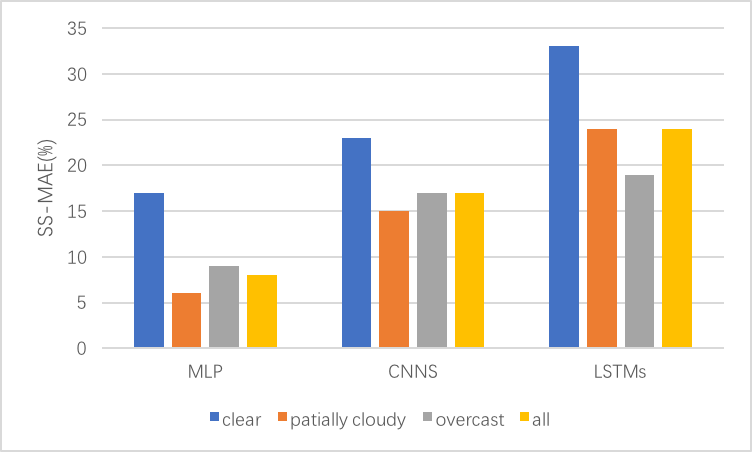
\includegraphics[width=0.8\textwidth]{ssmae.png}
	\caption{ss for mae\label{fig:lstm}}
\end{figure}






The figure 6.4 and figure 6.5 reveals that all the new constructed models all perform better than the baseline model as their scores all higher than 0.

For three weather conditions, the mae skill scores of CNN are all higher than MLP. For the 4 different situations, ss-mae of CNNs improves 6\%,9\%,8\%,9\% respectively.
It reveals that the image information is of great help to improve the performance of model.
LSTMs has the greatest gain in these three models.The skill scores of LSTMs reach 33\%,24\%,19\%,24\% respectively, which indicates that the  temporal characteristic combines with and image information can make better prediction than CNNs.




\begin{figure}[!ht]
	\centering
	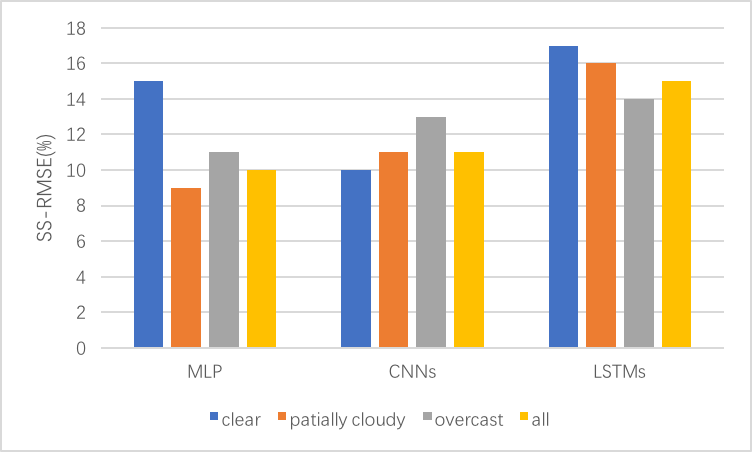
\includegraphics[width=0.8\textwidth]{ssrmse.png}
	\caption{ss for rmse\label{fig:lstm}}
\end{figure}


For three weather conditions, the rmse skill scores of CNN are also higher than MLP. For the 4 different situations, ss-mae of CNNs improves 5\%,2\%,2\%,1\% respectively.LSTMs is also the best in these three models.The skill scores of LSTMs reach 17\%,16\%,14\%,15\% respectively. The combination of  temporal characteristic and image information can make better prediction.






% {Description of the results followed by their review. These may include, where appropriate, feedback from test groups, users and the project sponsor.}


\chapter{Conclusions}
\section{Summary}

The prediction of photovoltaic values can reduce the impact of these unfavorable factors on the grid, which is beneficial to provide important support for power grid scheduling, decision-making and effective reduction for the operating cost of power system. 
However, estimating PV based on the relative position of sun and cloud, however, is quite challenging because of the changing weather patterns.
Therefore, this thesis proposed three different neural network models (MLP, CNNs, LSTMs) to solve this problem. The specific work content of the thesis is as follows.


1.This article explains the advantages and significance of photovoltaic power generation. It discusses the existing methods of predicting photovoltaic power generation and points out the advantages and disadvantages of the method.

2. The data source and the form of data generation are well explained. It also discusses 3 different neural networks that this article intends to adopt. The characteristics and advantages of three types of networks are also analyzed.

3. The steps and methods of preprocessed power values and sky images are specifically introduced.At the same time, the model structure of three different networks used in this paper is explained.Then the loss function used by neural networks has been introduced.

4 According to different weather, the preprocessed data is divided into three parts, which  uses the data as the input of the neural network to train the network. The experimental results show that the error of LSTMs is the smallest, and the effect is relatively best among the three models.



\section{Limitation}
This thesis merely discusses 3 different networks to predict the power values. This project still has several limitations.

Firstly, one of the limitations of this work is that there is only data for one month, which is not rich in weather changes and does not cover some extreme weather conditions.
Secondly, network training adopts the gray image of single channel, which will lose part of feature.As a result, the model is not accurate in extracting image features.

Thirdly, in CNN network structure, vgg net is adopted. However, other structures of CNN also have good performance.Therefore, other deep network structure models can be considered.




\section{Prospects for Further Work}


As for future works, Firstly,  the data set can be expanded through collecting sky images and corresponding power value of weather conditions. If the network has rich dataset, the prediction results are more generalized.

Secondly, when acquiring image information, visual attention can be used to better obtain image features. Besides, tasks can be decomposed to design different network structures (or branches) to focus on different sub-tasks, so as to redistribute the learning ability of the network and reduce the difficulty of original tasks and make the network easier to train.

Thirdly, the CNN network of models in this project  is VggNet. The structure of VggNet can be changed to ResNet for the network training test and prediction effect because ResNet has better performance than VggNet in image classification field.









% Switch back to single spacing so things don't look so ugly in these sections
\singlespacing

% Don't forget to supply a dissertation.bib file with your bibliography in
% BibTex format




\addcontentsline{toc}{chapter}{References Cited}

\bibliographystyle{ieeetr}
\bibliography{wp_ref}




\end{document}
